\documentclass[11pt,a4paper]{article}
\usepackage[T1]{fontenc}
\usepackage[utf8]{inputenc}
\usepackage{lmodern,microtype}
\usepackage[margin=25mm,headheight=15pt]{geometry}
\usepackage{amsmath,amssymb,amsthm,mathtools}
\usepackage{booktabs,longtable,array,enumitem}
\usepackage{xcolor,graphicx,fancyhdr,needspace}
\usepackage{xurl}
\usepackage[colorlinks=true,linkcolor=blue!45!black,urlcolor=blue!50!black,citecolor=blue!45!black]{hyperref}
\usepackage{bookmark}
\definecolor{ink}{RGB}{27,46,65}
\definecolor{accent}{RGB}{0,105,115}
\pagestyle{fancy}\fancyhf{}
\fancyhead[L]{\small Constructive general topology}
\fancyhead[R]{\small iPRA}\fancyfoot[C]{\thepage}
\setlength{\parskip}{4pt}
\setlength{\parindent}{1.1em}
\setlength{\emergencystretch}{3em}
\setlist{itemsep=3pt,topsep=5pt}
\newtheorem{theorem}{Theorem}[section]
\newtheorem{lemma}[theorem]{Lemma}
\newtheorem{proposition}[theorem]{Proposition}
\newtheorem{corollary}[theorem]{Corollary}
\theoremstyle{definition}
\newtheorem{definition}[theorem]{Definition}
\newtheorem{remark}[theorem]{Remark}
\newcommand{\N}{\mathbb N}
\newcommand{\Z}{\mathbb Z}
\newcommand{\Q}{\mathbb Q}
\newcommand{\R}{\mathbb R}
\newcommand{\ipra}{\ensuremath{\mathsf{iPRA}}}
\newcommand{\Ftwo}{\mathbb F_2}
\newcommand{\code}[1]{\texttt{#1}}
\newcolumntype{P}[1]{>{\raggedright\arraybackslash}p{#1}}
\hypersetup{pdftitle={General topology in intuitionistic primitive recursive arithmetic},pdfauthor={Research report prepared for Vladimir Reshetnikov}}
\begin{document}
\hypersetup{pageanchor=false}
\begin{titlepage}
\vspace*{15mm}
{\color{accent}\large CONSTRUCTIVE MATHEMATICS / EXPLICIT FINITE PROOFS\par}
\vspace{12mm}
{\color{ink}\Huge\bfseries General topology in intuitionistic primitive recursive arithmetic\par}
\vspace{8mm}
{\Large Finite spaces, quantitative metric constructions, homology, dimension, and approximate hairy-ball theorems\par}
\vspace{13mm}
{\large Prepared for Vladimir Reshetnikov\par}
{\large 19 November 2026\par}
\vfill
\begin{abstract}
We develop constructive arithmetic versions of theorems and structures linked directly from MathWorld's General Topology index. The treatment includes finite topology and separation, an exact finite compact-open exponential law, quantitative Urysohn separation and Hilbert-cube embeddings, equipped products and compact function spaces, finite homology and sheaves, a rational-grid proof of dimension invariance, and a finite-chain proof of approximate hairy-ball theorems. Every infinite construction is supplied with explicit computational data and is interpreted as a first-order schema or a theorem about finite tables. A separate analysis explains why arbitrary-cover compactness, exact point selection, and unrestricted countable unions cannot simply be imported.
The human-readable proofs and their primitive recursive bounds are the main result. The archive also includes compiled Lean foundations, explicitly labeled formalization blueprints, executable exact-arithmetic checks, and a source-by-source scope ledger. It does not claim a completed object-language \code{Prf PRAAx} formalization of the entire collection.
\end{abstract}
\vspace{8mm}
{\small Source baseline: \code{VladimirReshetnikov/ProveIt}, commit\\
\code{eb8eb6653c85aa44f1e18dd4efa243f41b5a9e98}.}
\end{titlepage}
\hypersetup{pageanchor=true}
\tableofcontents
\newpage
\section{What is proved, and what the source actually asks}
\label{sec:scope}

The source is the \emph{direct list of 33 entries} on MathWorld's General Topology topic page \cite{MWIndex}. It is not a finite syllabus of 33 theorems. Several entries define terminology; others describe whole subjects, and Kirby's List is a collection of problems. We therefore fix the direct-link scope. Following every link recursively would include much of mathematics and many open problems.

The report gives precise replacements, not a claim that all of classical topology is a theorem of first-order arithmetic. Finite spaces and finite complexes are genuine mathematical spaces, not approximations to every space. Equipped metric presentations give a second, substantially broader class. Quantitative Euclidean dimension and approximate sphere results supply infinite-space applications whose proofs only inspect finite data.

\subsection{The principal results}

The finite chapter proves the topology--preorder correspondence, exact formulas for interior and closure, continuity as monotonicity, subspaces and quotient constructions, connected components, separation criteria, finite Urysohn and Tietze extension theorems, metrization and quasi-metrization, finite products, and the compact-open exponential law.

The metric chapter proves explicit product-net estimates, distance-function Urysohn separation, quantitative coordinate metrization and Hilbert-cube embedding, and finite-mesh control of function-space distance, approximate extrema, evaluation and currying. Hypotheses include the relevant moduli, locators, base points, or separation information; they are not silently extracted from arbitrary classical topologies.

Finite linear algebra yields Betti numbers, Euler--Poincare, chain-homotopy invariance, collapses, and the usual genus formulas for explicitly presented polygonal cell complexes. Finite sheaf gluing and stalks, finite Boolean algebras, and graph coloring provide further direct connections to the index.

Two longer arguments deserve emphasis:
\begin{itemize}
\item A rational table on a $d$-cube whose opposite faces remain $h$ apart cannot land in fewer than $d$ coordinates while every Kuhn simplex has image diameter less than $h/d$. A bounded procedure returns an explicit violation. This proves dimension invariance for locally uniformly equipped homeomorphisms.
\item A finite chain calculation separates the identity from the antipodal map on an even-dimensional sphere. With explicit Lipschitz data, it produces approximate zeros of tangent fields by a bounded rational search. On odd-dimensional spheres a nonvanishing tangent field is given explicitly.
\end{itemize}

\subsection{Three distinctions that prevent false conclusions}

\paragraph{Constructive mathematics versus the strength of \ipra.}
A proof may avoid classical logic and still use induction or recursion beyond primitive recursive arithmetic. We give bounds and quantifier-free loop invariants. Conversely, enormous finite searches are permitted: computational practicality is not the criterion.

\paragraph{Semantic Lean theorems versus embedded arithmetic derivations.}
A Lean theorem about natural numbers, preorders, or metric structures is not by itself a proof that an object-language sentence is derivable in \ipra. The latter requires a term of the form
\[
([]:\operatorname{List}(\operatorname{Fm}\ \operatorname{PTm}\ 0))
 \ \vdash[\operatorname{PRAAx}]\ \varphi.
\]
The archive's checked foundation lemmas and its planned object-language endpoints are identified separately. No placeholder is presented as a completed topology theorem.

\paragraph{Verification of a certificate versus production of a certificate.}
Checking an embedded disk, a finite cover, or a chain contraction does not establish that every classical instance admits such a certificate within a primitive recursive bound. Where production is proved, an algorithm and bound are provided. Where only verification is available, the conclusion is conditional and is labeled accordingly.

\subsection{Two corrections to the source scope}

The entry named \emph{Compactness Theorem} concerns bounded rectifiable currents and the flat norm \cite{MWCurrents}; it is neither logical compactness nor merely the compactness of closed intervals. Section~\ref{sec:limits} proves a fixed-mesh chain replacement and identifies the missing uniform deformation and closure arguments.

The wording on the \emph{Dehn's Lemma} page omits a necessary restriction \cite{MWDehn}. A null-homotopic simple closed curve in the \emph{boundary} of a 3-manifold bounds an embedded disk under the standard hypotheses. Another usual formulation requires a singular disk with no singularities along its boundary. A merely embedded loop in the interior that extends continuously to a disk is insufficient: every knot in $\R^3$ is null-homotopic, but a nontrivial knot does not bound an embedded disk there. We use the correctly restricted target, and prove only an explicit bounded certificate version in this packet. The boundary formulation is also stated in the topology literature \cite{DehnPrimary}.

\subsection{Coverage of the direct index}

The following table states mathematical scope, not formal completion. The machine-readable source map retains all 33 individual page URLs.
\begin{longtable}{P{.28\textwidth}P{.64\textwidth}}
\toprule
Index entries & Treatment in this report\\
\midrule
\endhead
Topology; Exterior; Local &
Finite topologies, interior/closure/exterior, least neighborhoods and local tests; finite family tests.\\
Homeomorphic; Homeomorphism &
Finite preorder isomorphisms, explicit inverses and invariants; equipped Euclidean dimension obstruction.\\
Homeomorphic Type &
Invariants of supplied standard surface presentations; the full surface-classification theorem is not proved.\\
Euclidean Topology; Dimension; Dimension Invariance Theorem &
Rational grids, explicit norm comparison, finite obstruction and modulated homeomorphisms.\\
Urysohn's Lemma &
Finite normal spaces; distance functions with positive denominators and explicit moduli.\\
Urysohn's Metrization Theorem &
Finite metrization and quasi-metrization; equipped separating coordinates and a metric Hilbert-cube embedding.\\
Tychonoff Theorem &
Finite-space compact products and equipped finite/countable metric product nets; no arbitrary-cover theorem.\\
Compact-Open Topology &
Finite exact exponential law and quantitative compact-domain function-space constructions.\\
Betti Number; Euler Characteristic; Genus &
Rational finite chain complexes, invariance under supplied chain homotopies, certified surface cell presentations.\\
Hairy Ball Theorem &
Explicit odd-sphere field, linear-field obstruction, finite antipodal obstruction, bounded approximate zeros on even spheres.\\
Coloring &
Finite graph coloring, bipartite criterion and the graph Betti-number formula.\\
Presheaf of Categories &
Finite category/functor diagram interface; no higher-category descent theorem.\\
Restriction Map; Restriction of a Sheaf; Sheaf; Sheaf of Rings; Sheaf Section; Stalk; Subsheaf &
Finite presheaves, unique gluing, restrictions, minimal-neighborhood stalks and pointwise ring operations.\\
Sigma-Algebra &
Finite Boolean algebras and atoms; bounded or stabilization-certified unions; an unbounded-union obstruction.\\
Sigma-Discrete Family; Sigma-Locally Finite Family &
Finite-prefix tests and supplied local-support bounds. No arbitrary infinite support extractor.\\
Compactness Theorem &
Fixed-mesh bounded integral chains and a conditional finite-scale deformation consequence.\\
Dehn's Lemma &
Bounded PL disk certificates and their exact verification, not general disk-existence production.\\
Differential Topology &
The tangent-field results above; no claim to cover the entire subject.\\
Kirby's List &
Classified as a problem collection, not asserted or solved.\\
\bottomrule
\end{longtable}

\subsection{How ProveIt is reused}

The source snapshot is commit \code{eb8eb6653c85aa44f1e18dd4efa243f41b5a9e98}. Its main README explicitly distinguishes the checked \code{ConciseIPRA}, \code{Derivations}, and \code{Bridge} libraries from delivered research packets that have not been rerun or verified \cite{RepoReadme}. We follow that distinction.

The fixed-symbol/finite-table discipline and observation-carrier viewpoint agree with the existing topology framework \cite{RepoTopology}. The dimension chapter reconstructs the argument in the existing dimension-invariance packet, including its essential staggered-grid idea \cite{RepoDimension}. It is reuse with a fresh explanation and additional integration, not a novelty claim. The native transfer interface is the inspected \code{pra\_iff\_native} theorem \cite{RepoNative}. It transfers an already constructed arithmetic proof; it does not manufacture one from an external mathematical assertion.


\section{Arithmetic foundation and representation contracts}
\label{sec:arithmetic}

\subsection{The theory}

We use first-order intuitionistic logic with equality. The numerical language contains $0$, successor, and symbols for each \emph{fixed} primitive recursive definition needed in a theorem. The nonlogical axioms are successor injectivity, successor distinct from zero, the defining equations for composition and primitive recursion, and quantifier-free induction:
\[
 \bigl(A(0,\vec a)\wedge
   \forall t(A(t,\vec a)\to A(t+1,\vec a))\bigr)
       \longrightarrow \forall t\,A(t,\vec a),
\]
where $A$ is quantifier-free. Ordinary intuitionistic natural-deduction rules, equality reflexivity and substitution are the logical rules. Finite conjunctions, disjunctions and implications are allowed in a quantifier-free formula; bounded quantifiers in the exposition are compiled into primitive recursive Boolean folds before induction is applied.

This is the ordinary \ipra\ interface used by the inspected ProveIt libraries \cite{RepoReadme,RepoNative}. The report does not add excluded middle for arbitrary formulas, countable choice, a power-set sort, a real-number sort, or induction for arbitrary arithmetic formulas.

\subsection{Concrete finite codes}

One possible pairing code is
\[
 \langle a,b\rangle=2^a(2b+1)-1.
\]
For a code $z$, its two projections are recovered by bounded division and a bounded search below $z+1$. Lists carry an explicit length and an iterated pairing of their entries; invalid or truncated codes decode to default values. Signed integers use the zigzag code
\[
 0\mapsto0,\qquad t>0\mapsto2t,\qquad -t\mapsto2t-1.
\]
A rational is a pair $(a,b)$ with $a\in\Z$, $b\in\N_{>0}$; reduction by a gcd is optional. Equality and order are decided by cross-multiplication. Division by zero is totalized to zero and accompanied by a validity guard whenever its intended meaning is used.

A subset of $\{0,\ldots,n-1\}$ is a mask below $2^n$. A binary relation is a mask below $2^{n^2}$. A finite complex is a family of masks closed under taking submasks. A rational matrix is a list of row lists with checked dimensions. Every displayed bounded operation on these codes is primitive recursive, including exponentiation, finite sums, permutations, integer determinants, and rational Gaussian elimination.

\begin{lemma}[Finite decision and witness extraction]\label{lem:bounded-search}
For a fixed primitive recursive Boolean predicate $p(a,i)$ and a supplied bound $B(a)$, the conjunction and disjunction over $i<B(a)$ are primitive recursive. If the disjunction is $1$, a primitive recursive least-index scan returns an $i<B(a)$ with $p(a,i)=1$. If the scan fails, every entry is $0$.
\end{lemma}
\begin{proof}
Set $c(0)=1$ and $c(t+1)=c(t)p(a,t)$ for conjunction, and use Boolean or for disjunction. The witness scan maintains a flag and the first successful index, retaining a default index $B(a)$ until success. Its state after step $t$ is computed by primitive recursion.

For a free index $j$, quantifier-free induction verifies the guarded assertions that a recorded index lies below the processed prefix, satisfies $p=1$, and has all preceding tests zero; the last condition is itself a Boolean fold. The failure flag equals the conjunction of the negated processed tests. These are equations and bounded order tests on the state. Reading the terminal invariant proves the claims. Extracting a witness from a nonzero \emph{finite} disjunction uses no unbounded double-negation elimination.
\end{proof}

\begin{lemma}[Verified bounded-loop rule]\label{lem:loop-rule}
Let $s_0(a)$, $S(t,s,a)$, and $T(a)$ be fixed primitive recursive functions. Suppose a quantifier-free predicate $I(t,s,a)$ has an \ipra\ proof of its initial case and of preservation under $S$ for $t<T(a)$. Then \ipra\ proves $I(T(a),s(T(a),a),a)$ for the primitive recursive run
\[
s(0,a)=s_0(a),\qquad s(t+1,a)=S(t,s(t,a),a).
\]
Any quantifier-free output consequence therefore has an \ipra\ proof.
\end{lemma}
\begin{proof}
Apply quantifier-free induction to
$t\leq T(a)\to I(t,s(t,a),a)$, using the defining equations of $s$. The guard is a characteristic-function equation. Instantiate the result at $T(a)$ and use the terminal consequence. This rule assumes actual proofs of the invariant conditions; it does not assert that every true program specification is provable.
\end{proof}

\subsection{First-order schemas for infinite objects}

A map on an infinite metric space is not quantified over as an arbitrary set-theoretic function inside \ipra. There are three accepted interfaces:
\begin{enumerate}
\item Fix the primitive recursive syntax trees of an evaluator and its moduli, and prove a theorem in the numerical parameters. This is a \emph{schema} indexed externally by fixed definitions.
\item Give a finite observation table, its dimensions, and a Boolean validity predicate. The theorem is uniform in the table code.
\item Give a program together with an explicit finite time bound and trace. Verify the trace by a bounded scan. The theorem is conditional on that trace, unless its production has separately been proved.
\end{enumerate}

There cannot be a total primitive recursive evaluator $U(e,x)$ for all primitive recursive programs: $x\mapsto U(x,x)+1$ would itself have an index $d$, contradicting its value at $d$. The distinction matters for countable products, dense sequences, moduli and families of matrices. Each fixed uniform family used below must have a fixed joint evaluator; a list of arbitrary PR program codes is not enough.

\begin{definition}[Rational real-name convention]
A real name is a fixed rational evaluator $q(k)$ with a certified estimate
\[
 |q(k)-q(\ell)|\leq 2^{-k}+2^{-\ell}.
\]
Semantic notation $x=\lim_kq(k)$ abbreviates the corresponding rational approximation assertions. A displayed inequality involving named reals is used internally through rational approximants with explicit error slack. Finite-dimensional vectors use coordinatewise names and the sup norm.
\end{definition}

For a metric presentation, the same convention applies to $d(x,y)$, and the distance laws are supplied as arithmetic approximation contracts. A continuity modulus $\mu$ specifies, with a fixed convention,
\[
 d(x,y)\leq2^{-\mu(k)}
   \quad\Longrightarrow\quad d(fx,fy)\leq2^{-k}.
\]
An inverse modulus, net locator or distance-to-set evaluator is additional data. It is never inferred merely from the negation of a counterexample.

A countable name need not be collected into an actual set in the object language. To prove an assertion at precision $k$, the proof computes all required precision and index bounds first, builds the finite table, verifies its inequalities, and concludes the requested arithmetic statement. Universal quantification over $k$ comes after this finite construction.

\subsection{What approximate existence means}

A theorem
\[
 \forall k\ \exists w\ R(k,w)
\]
with a primitive recursive witness $w=W(k)$ and bounded $R$ is meaningful positive information. It does not imply that the witnesses are a coherent Cauchy sequence, nor that an exact root or fixed point has a primitive recursive name. A sequence of near-maximizers, for example, can alternate between distant maxima. The metric and sphere chapters carefully distinguish an approximate witness from an exact selected point.

Total boundedness is a net construction. Completeness requires a specified way to interpret a Cauchy name with a modulus. Arbitrary open-cover compactness, sequential compactness without a convergence modulus, and total boundedness are not interchangeable in this constrained setting.

\subsection{Induction audit used throughout}

The arithmetical proof cores below use the verified-loop rule and fixed finite algebra. The relevant invariants are given where a nontrivial construction appears. The common patterns are:
\begin{center}
\begin{tabular}{P{.29\textwidth}P{.60\textwidth}}
\toprule
Construction & Quantifier-free invariant after bounded expansion\\
\midrule
Relation closure & The current table contains exactly paths of length at most the current bound.\\
Finite topology tests & The Boolean accumulator equals the tested prefix of the topology or separation axioms.\\
Gaussian elimination & Elementary matrices give the current matrix from the original; completed pivot rows have the required zeros.\\
Chain and prism sums & Each coefficient equals its processed incidence sum; interior terms cancel in matched pairs.\\
Dimension parity & The parity for a fixed restricted labeling equals its previous-face parity.\\
Product nets & The constructed tuple covers the already processed coordinates; the remaining tail has a numerical bound.\\
Barycentric refinement & Every resulting simplex lies in its parent and obeys the stated mesh estimate.\\
Finite sheaf gluing & The partial tuple agrees on all processed overlaps.\\
\bottomrule
\end{tabular}
\end{center}
These are plans for object-language proofs with explicit witnesses and bounds, backed by the human arguments. They are not a claim that all such proofs have already been constructed in Lean.


\section{Finite topology as primitive recursive mathematics}\label{sec:finite}

This section proves twenty-four uniform finite theorems.  They address the
entries on topology, exterior, homeomorphisms, compact-open topology,
Urysohn separation and metrization, together with finite forms of the
discrete-family terminology.  The restriction is on the \emph{represented
objects}, not on the sizes of the finite instances: the proofs are uniform
in every natural-number carrier size.  All subsets here have Boolean
codes.  Consequently bounded searches, complement formation, and
case distinctions on membership are legitimate in \ipra.  Nothing in
this section turns an arbitrary infinite predicate into a decidable set.

\subsection{Codes and the specialization relation}

Put $[n]=\{0,\ldots,n-1\}$.  A subset $A\subseteq[n]$ is represented by
the integer $a<2^n$ whose $x$th binary digit is its membership bit.  A
relation is represented by $r<2^{n^2}$; write $x\preceq y$ when bit
$nx+y$ is one.  Its validity conditions are the bounded statements
\[
 (\forall x<n)\ x\preceq x,\qquad
 (\forall x,y,z<n)\bigl(x\preceq y\land y\preceq z
                         \Rightarrow x\preceq z\bigr).
\]
They define a \emph{preorder}; antisymmetry is not required.  A topology
table is a mask of length $2^n$: its bit at $a$ says whether the subset
with code $a$ is open.  A map $[n]\to[m]$ is a length-$n$ table of
entries below $m$.  Empty carriers cause no exception: there is one
empty table, and there is no map from a nonempty carrier to the empty
one.

For a preorder define
\[
 \mathord\uparrow x=\{y:x\preceq y\},\qquad
 \mathord\downarrow x=\{y:y\preceq x\}.
\]
A set $U$ is \emph{upward closed} if $x\in U$ and $x\preceq y$ imply
$y\in U$; downward closed has the reversed implication.  The chosen
orientation is important: open sets will be upward closed, and the
closure of $\{x\}$ will be $\mathord\downarrow x$.

\begin{theorem}[F01: topology from a preorder]\label{thm:finite-upsets}
The upward-closed subsets of a finite preorder form a topology.
The least open neighborhood of $x$ is $\mathord\uparrow x$, and these
$n$ sets form a basis.  Every open set $U$ satisfies
$U=\bigcup_{x\in U}\mathord\uparrow x$.
\end{theorem}
\begin{proof}
The empty and full sets are upward closed.  If $x$ belongs to both of
two upward-closed sets, every $y$ above $x$ belongs to both; hence their
intersection is upward closed.  If $x$ belongs to a member of a coded
family, that same member contains every $y$ above $x$; its union is
therefore upward closed.  Transitivity makes
$\mathord\uparrow x$ upward closed, reflexivity puts $x$ in it, and
the definition of upward closure places it in every open neighborhood
of $x$.  These observations prove the displayed union identity.
For the finite topology table, closure under binary unions already
gives closure under every finite list by a bounded fold.  No code for
an unbounded union is required.
\end{proof}

\begin{theorem}[F02: recovery of every finite topology]\label{thm:finite-recover}
Suppose a table $\mathcal T$ contains the empty and full subsets and
is closed under binary intersection and union.  Define
\[
 x\preceq_{\mathcal T}y
 \quad\Longleftrightarrow\quad
 (\forall U\in\mathcal T)\ (x\in U\Rightarrow y\in U).
\]
This is a preorder, and its upward-closed subsets are exactly
$\mathcal T$.  Starting with a preorder and performing this recovery
returns the original relation.
\end{theorem}
\begin{proof}
Reflexivity and transitivity follow by substituting the same open set
into the defining implications.  Let $N_x$ be the intersection of
the at most $2^n$ listed opens containing $x$.  This nonempty list
includes $[n]$, so a bounded fold computes $N_x\in\mathcal T$.
Its elements are exactly the $y$ with $x\preceq_{\mathcal T}y$.
Every listed open is upward closed by definition.  Conversely, an
upward-closed $U$ is the union of $N_x$, $x\in U$, so belongs to
$\mathcal T$ by binary-union closure.  Finally, for an initial
preorder, $x\preceq y$ implies membership of $y$ in every upward
set containing $x$.  If the recovered relation holds, apply it to
the upward set $\mathord\uparrow x$ to recover $x\preceq y$.
All quantifiers in this construction run over bounded mask ranges.
\end{proof}

\subsection{Interior, closure, exterior, and boundary}

\begin{theorem}[F03: explicit interior and closure]\label{thm:finite-intcl}
For every coded subset $A$,
\[
 \operatorname{Int}A=\{x:(\forall y<n)(x\preceq y\Rightarrow y\in A)\},
 \qquad
 \operatorname{Cl}A=\{x:(\exists y<n)(x\preceq y\land y\in A)\}.
\]
The first is the greatest open subset of $A$, and the second is the
least closed superset of $A$.  Here closed subsets are exactly the
downward-closed subsets.
\end{theorem}
\begin{proof}
A complement is upward closed exactly when the original set is
downward closed, by decidable membership.  Reflexivity shows
$\operatorname{Int}A\subseteq A\subseteq\operatorname{Cl}A$.
If $x$ satisfies the universal condition and $x\preceq z$, then
every $y$ above $z$ is above $x$, so $z$ also satisfies it.  Thus the
interior formula defines an open set.  If $U$ is open and
$U\subseteq A$, every point above $x\in U$ remains in $U$ and hence
in $A$; therefore $U\subseteq\operatorname{Int}A$.
If $z\preceq x$ and $x\preceq y\in A$, transitivity gives
$z\preceq y\in A$, proving that the closure formula is downward
closed.  Any downward-closed $D\supseteq A$ contains such $x$, so it
contains $\operatorname{Cl}A$.  Both formulas are evaluated by loops
of length at most $n^2$.
\end{proof}

\begin{theorem}[F04: closure and interior laws]\label{thm:finite-laws}
Interior and closure are monotone and idempotent.  Moreover,
\[
\begin{split}
 \operatorname{Int}(A\cap B)&=\operatorname{Int}A\cap\operatorname{Int}B,\\
 \operatorname{Cl}(A\cup B)&=\operatorname{Cl}A\cup\operatorname{Cl}B,\\
 \operatorname{Int}(A^c)&=(\operatorname{Cl}A)^c,\qquad
 \operatorname{Cl}(A^c)=(\operatorname{Int}A)^c.
\end{split}
\]
Also $\operatorname{Cl}\varnothing=\varnothing$ and
$\operatorname{Int}[n]=[n]$.
\end{theorem}
\begin{proof}
Monotonicity follows by retaining a universal membership proof or an
existential witness when $A$ is enlarged.  Since the interior is
already open, its greatest-open characterization gives idempotence;
the least-closed characterization gives the dual assertion.  A point
has every successor in $A\cap B$ exactly when every successor is
in each factor.  A successor in $A\cup B$ witnesses one of the two
closure alternatives, and either alternative witnesses the union.
The first complement identity says that no successor lies in $A$;
this is precisely the failure of the existential condition for
closure.  For the second identity, if the bounded universal test
fails, a scan of the $n$ entries returns a successor outside $A$.
This last step uses decidability and finiteness, not a De Morgan
principle for arbitrary predicates.  Empty and full sets follow
directly from the formulas.
\end{proof}

\begin{theorem}[F05: exterior and boundary decomposition]\label{thm:finite-boundary}
Define $\operatorname{Ext}A=\operatorname{Int}(A^c)$ and
$\partial A=\operatorname{Cl}A\cap\operatorname{Cl}(A^c)$.
Then
\[
 [n]=\operatorname{Int}A\ \dot\cup\ \partial A\ \dot\cup\
             \operatorname{Ext}A,
 \qquad
 \partial A=\operatorname{Cl}A\setminus\operatorname{Int}A.
\]
The boundary is closed and $\partial A=\partial(A^c)$.
A subset is both open and closed exactly when its boundary is empty.
\end{theorem}
\begin{proof}
By F04, the exterior is the complement of the closure and
$\operatorname{Cl}(A^c)$ is the complement of the interior.
Since interior is contained in closure, the three indicated Boolean
pieces are disjoint and cover the carrier.  The boundary is an
intersection of closed sets and its definition is symmetric in $A$
and $A^c$.  If $A$ is clopen, its interior and closure are both $A$.
Conversely, empty boundary gives
$\operatorname{Cl}A\subseteq\operatorname{Int}A$; sandwiching $A$
between these sets makes all three equal.
\end{proof}

\subsection{Maps and universal constructions}

\begin{theorem}[F06: continuity is monotonicity]\label{thm:finite-cont}
A map $f:X\to Y$ between finite preorder spaces is continuous
exactly when $x\preceq_X x'$ implies $f(x)\preceq_Y f(x')$.
Identity maps and composites of continuous maps are continuous.
\end{theorem}
\begin{proof}
For a monotone map the inverse image of an upward set is upward:
if $f(x)\in U$ and $x\preceq x'$, then
$f(x)\preceq f(x')$ puts $f(x')$ in $U$.
Conversely, take the open neighborhood
$\mathord\uparrow f(x)$ of $f(x)$.  Its inverse image is open
and contains $x$, so contains every $x'$ above $x$.  This says
$f(x)\preceq f(x')$.  The identity preserves the relation, and
two successive relation-preserving implications prove the composite
claim.  A continuity certificate can therefore be checked using
$|X|^2$ comparisons instead of enumerating all subsets of $Y$.
\end{proof}

\begin{theorem}[F07: the closure criterion]\label{thm:finite-closuremap}
A finite map $f:X\to Y$ is continuous if and only if
\[
 f(\operatorname{Cl}_X A)\subseteq\operatorname{Cl}_Y f(A)
 \quad\hbox{for every coded }A\subseteq X.
\]
\end{theorem}
\begin{proof}
For the forward implication, a witness $x\preceq a\in A$
is carried to $f(x)\preceq f(a)\in f(A)$.
For the converse, if $x\preceq y$, apply the displayed inclusion
to $A=\{y\}$.  The closure of $\{f(y)\}$ consists precisely of
the elements below $f(y)$, so $f(x)\preceq f(y)$; now use F06.
\end{proof}

\begin{theorem}[F08: homeomorphisms and classification]\label{thm:finite-homeo}
A bijection of finite spaces is a homeomorphism exactly when
\[
 x\preceq_X y\quad\Longleftrightarrow\quad f(x)\preceq_Y f(y).
\]
Homeomorphism is an equivalence relation and is decidable for finite
topology tables by a primitive recursive search.
\end{theorem}
\begin{proof}
The two implications are monotonicity of $f$ and of its inverse,
using the inverse table computed by bounded search.  F06 proves the
first assertion.  Identity, inverse, and composition prove
reflexivity, symmetry, and transitivity.  If the carrier sizes differ,
no bijection exists; if they agree, enumerate all $n^n$ tables,
discard those with repeated values, and check the two relation
implications.  This explicit bound suffices; a more efficient
permutation enumeration changes no logical issue.
\end{proof}

\begin{theorem}[F09: subspaces]\label{thm:finite-subspace}
For a coded $S\subseteq X$, restricting the preorder to $S$ gives
exactly the subspace topology.  If $A\subseteq S$, then
$\operatorname{Cl}_S A=S\cap\operatorname{Cl}_X A$.
\end{theorem}
\begin{proof}
An intersection of an upward set of $X$ with $S$ is upward for the
restricted relation.  Conversely, if $V\subseteq S$ is relatively
upward, let $U=\{y\in X:(\exists v\in V)\ v\preceq y\}$.
This set is upward, and $U\cap S=V$: one inclusion uses
reflexivity and the other relative upward closure.  The closure
formula in F03 quantifies over witnesses $a\in A$ in either space,
so intersecting the answer with $S$ proves the second assertion.
Enumerating the elements of $S$ increasingly gives a carrier
$[|S|]$ and an explicit relabeling table.
\end{proof}

\begin{theorem}[F10: finite products]\label{thm:finite-products}
The product topology on $X\times Y$ is the topology of
\[
 (x,y)\preceq(x',y')\quad\Longleftrightarrow\quad
 x\preceq_X x'\ \land\ y\preceq_Y y'.
\]
The projections are continuous, and a map into the product is
continuous exactly when its two components are continuous.  The
same assertions hold for any coded finite list of factors.
\end{theorem}
\begin{proof}
The least neighborhood of $(x,y)$ in the displayed preorder is
$\mathord\uparrow x\times\mathord\uparrow y$, a basic product
open.  Every product open is upward for the coordinate relation,
and these least neighborhoods express every upward set as a union
of product opens.  This proves equality of topologies.  The
universal property is the assertion that a pair of relation
implications holds exactly when each holds.  For finitely many
factors, iterate this construction using mixed-radix codes; the
carrier-size bound is the product of the factor sizes.  An empty
list has the one-point product, while an empty factor gives the
empty product carrier.
\end{proof}

\begin{theorem}[F11: quotient spaces]\label{thm:finite-quotients}
Let $q:X\twoheadrightarrow Y$ be a coded surjection of finite sets.
On $Y$ take the reflexive transitive closure of the generating edges
\[
 q(x)\longrightarrow q(x')\quad(x\preceq_X x').
\]
Its upward topology is the quotient topology.  A map $g:Y\to Z$
is continuous exactly when $gq$ is continuous.
\end{theorem}
\begin{proof}
A subset $V\subseteq Y$ is upward for every generating edge
exactly when $q^{-1}V$ is upward in $X$; upwardness for edges
extends along paths and hence along their reflexive transitive
closure.  This is the defining quotient-open condition.  Similarly,
a map preserves the closure relation exactly when it preserves
every generating edge; this is equivalent to monotonicity of
$gq$, and F06 concludes the proof.  The closure is computable by
Warshall's recurrence: at stage $k$ allow paths whose interior
vertices belong to $\{0,\ldots,k-1\}$, then add paths through $k$.
After $|Y|$ stages every path is covered.  Equivalently, deleting
repeated vertices reduces any reachable pair to a path of at most
$|Y|-1$ edges.  Both give primitive recursive bounds.
\end{proof}

\begin{theorem}[F12: the $T_0$ quotient]\label{thm:finite-tzero}
Put $x\sim y$ when $x\preceq y$ and $y\preceq x$.
The equivalence classes, ordered by $[x]\leq[y]$ when
$x\preceq y$, form a finite partial order.  Its quotient map
induces a bijection between open-set tables.  Every continuous map
from $X$ into a finite $T_0$ space factors uniquely through this
quotient.  A finite space is $T_0$ exactly when its preorder is
antisymmetric.
\end{theorem}
\begin{proof}
Reflexivity, symmetry, and transitivity of $\sim$ follow directly
from the preorder axioms.  Replacing either representative by an
equivalent one leaves the order implication unchanged by
transitivity; mutual order of two classes makes them equal.
Every upward set is constant on equivalence classes, so descent
and inverse image give mutually inverse operations on opens.
Two distinct classes are distinguished by a principal upward set:
if neither principal set distinguished them, the representatives
would be mutually below one another.  Conversely, equivalent
points have identical open neighborhoods, proving the $T_0$
characterization.  A monotone map into an antisymmetric relation
sends equivalent points to equal points, so descends uniquely;
its descended map is monotone.  Taking the least numbered member
of each class provides canonical representatives by an $n$-step
scan; no quotient-type choice is needed in the arithmetic coding.
\end{proof}

\subsection{Connectedness and separation}

Join $x$ and $y$ by an undirected edge when $x\preceq y$ or
$y\preceq x$.  A \emph{component} below means a connected component
of this finite comparability graph.  Reachability is a bounded
predicate: repeated vertices can be deleted from a path, leaving
at most $n-1$ edges.  One can instead iterate neighborhood expansion
$n$ times, with a bitmask of reached vertices as the loop state.

\begin{theorem}[F13: clopen sets and components]\label{thm:finite-components}
A subset of a finite space is clopen if and only if it is a union
of comparability components.  Thus the topological connected
components are exactly these graph components, each of which is
itself open and closed.
\end{theorem}
\begin{proof}
A clopen set is both upward and downward closed, so its membership
bit is unchanged along a comparability edge, and then along a
path.  It is therefore a union of components.  Conversely, a union
of components cannot lose membership along either orientation of
an edge, making it both upward and downward closed.  In a single
component, a nonempty clopen subset must contain every point
reachable from one of its points and is therefore the whole
component.  Hence that component is connected.  Distinct
components are separated by the component and its clopen
complement, proving maximality and the topological assertion.
\end{proof}

\begin{theorem}[F14: connected images and products]\label{thm:finite-connected}
The image of a connected finite space under a continuous map is
connected with its subspace topology.  The product of two nonempty
connected finite spaces is connected.  More generally, the
components of a finite product of nonempty factors are exactly
the products of their components.
\end{theorem}
\begin{proof}
A monotone map takes a comparability edge to a comparability edge
or an equality.  Mapping a path and deleting repetitions connects
any two image points.  F13 proves the image assertion.
In a product, hold the second coordinate fixed and follow a path
in the first coordinate; then hold the first fixed and follow one
in the second.  Each step is a product comparability step by
reflexivity in the stationary coordinate.  Thus a product of
components is connected.  Conversely, the coordinate projection
of a product path is a path with possible repetitions, so a path
cannot leave either coordinate component.  Induction over the
coded number of factors proves the last assertion.  The empty
product convention from F10 is consistent with this description.
\end{proof}

\begin{theorem}[F15: finite separation collapses]\label{thm:finite-tone}
For a finite space, the following are equivalent: $T_1$;
Hausdorff; discrete; and $x\preceq y$ implies $x=y$.
Every finite space is second countable, with the explicitly listed
principal-neighborhood basis.
\end{theorem}
\begin{proof}
In a $T_1$ space each singleton $\{y\}$ is closed, so
$\mathord\downarrow y=\{y\}$ by F03.  This eliminates every
nonidentity order pair.  Conversely, the identity relation makes
every subset upward closed and gives the discrete topology.
Distinct points of a discrete space have disjoint singleton
neighborhoods.  If a finite space is Hausdorff and $x\preceq y$
with $x\ne y$, every neighborhood of $x$ contains $y$ and hence
meets every neighborhood of $y$, contradicting separation.
The basis in F01 supplies second countability directly; it can be
padded with empty sets if a natural-number indexing is desired.
\end{proof}

\begin{theorem}[F16: finite cover extraction]\label{thm:finite-cover}
Given a coded list $(U_i)_{i<r}$ of subsets covering a coded
$S\subseteq[n]$, one can compute at most $|S|$ indices whose sets
still cover $S$.  In particular every finite space, and every
coded subset of it, has this finite compactness property.
\end{theorem}
\begin{proof}
Visit the points of $S$ in increasing order.  For each $x$ scan
$i<r$ and retain the least index satisfying $x\in U_i$; coverage
guarantees that the scan succeeds.  Remove duplicate indices.
Every visited point is covered by its retained choice, and there
are at most $|S|$ choices.  The loop has at most $nr$ membership
tests, followed by bounded duplicate deletion.  The proof applies
to any subsets, so in particular to open covers and relative open
covers.  If an enumerated infinite family is used instead, the
same extraction requires as input a finite bound or a table of
witness indices covering the points; this proposition does not
compute such witnesses from unbounded existential assertions.
\end{proof}

\begin{theorem}[F17: finite compact--Hausdorff bijections]\label{thm:finite-ch}
A continuous bijection from a finite space onto a finite Hausdorff
space is a homeomorphism.  Its inverse table is primitive recursive
in the input tables.
\end{theorem}
\begin{proof}
By F15 the target is discrete.  Continuity makes the preimage of
each target singleton open, and bijectivity identifies these
preimages with all source singletons.  Thus the source is also
discrete, so the inverse is continuous.  For each target element
its unique preimage is found by scanning the source table.
F16 supplies the finite compactness premise familiar from the
general compact--Hausdorff theorem, but the finite proof above
does not require any infinite compactness principle.
\end{proof}

We use \emph{normal} in the convention of the MathWorld Urysohn
entry: any two disjoint closed sets have disjoint open
neighborhoods; $T_1$ is not silently included.  This convention
retains nontrivial finite examples.

\begin{theorem}[F18: exact finite normality criterion]\label{thm:finite-normal}
A finite preorder space is normal if and only if every
comparability component has a least equivalence class for
$\sim$ from F12.  Equivalently, for every component $C$ there is
$b\in C$ with $b\preceq x$ for every $x\in C$.
\end{theorem}
\begin{proof}
First pass to the finite partial order of equivalence classes;
its open and closed sets correspond exactly to the original ones.
Every element $x$ has a minimal element below it.  To see this
with a finite bound, begin at $x$ and replace the current element
by a strictly smaller one if possible.  A strict descending list
has no repeated element, so fewer than the number of classes
replacements are possible.  Every test and choice is bounded.

Suppose normality holds.  Two distinct minimal classes $a,b$
below the same $x$ have disjoint closed principal ideals
$\mathord\downarrow a=\{a\}$ and
$\mathord\downarrow b=\{b\}$.  Every open neighborhood of
either contains $x$, contradicting normality.  Consequently
each $x$ has a unique minimal class below it.  If $x\leq y$,
the minimal class below $x$ also lies below $y$, so the two
minimal classes are equal.  Following comparability paths shows
that this class is constant on a component, and lies below
every point there.  Lifting representatives proves necessity.

Conversely, choose a least class in each component.  If a closed
set meets a component, downward closure forces it to contain
that component's least class.  Hence two disjoint closed sets
$A,B$ cannot both meet a component.  The union of all components
meeting $A$ is clopen by F13, contains $A$, and misses $B$.
Its complement is a disjoint open neighborhood of $B$, proving
normality.  A directly checkable algorithm enumerates components
and searches their at most $n$ points for an element below every
point in that component.
\end{proof}

\begin{theorem}[F19: a two-valued finite Urysohn lemma]\label{thm:finite-urysohn}
In a finite normal space, disjoint closed coded sets $A,B$ admit
a continuous map $f:X\to\{0,1\}$, with the discrete topology,
such that $f|_A=0$ and $f|_B=1$.  Regard the values as rational
points of $[0,1]$ to obtain the usual Urysohn conclusion.
Conversely, the existence of such two-valued separators for all
disjoint closed pairs implies normality.
\end{theorem}
\begin{proof}
Let $C_A$ be the union of comparability components meeting $A$.
By the proof of F18 it is clopen and disjoint from $B$.  Set
$f(x)=0$ on $C_A$ and $f(x)=1$ elsewhere.  Both fibers are
open, so the inverse image of every subset of $\{0,1\}$ is open.
This proves continuity and the required values, including the
cases when one or both closed sets are empty.  For the converse,
the inverse images of $\{0\}$ and $\{1\}$ under a separator are
disjoint open neighborhoods.  In the usual interval formulation,
one may instead take inverse images of disjoint neighborhoods of
$0$ and $1$.

The entire output is a Boolean table obtained by graph
reachability and a scan for intersections with $A$; no real limit
is needed.  This is an exact finite specialization of the named
lemma, with a stronger conclusion about the function's range.
\end{proof}

\begin{theorem}[F20: finite rational Tietze extension]\label{thm:finite-tietze}
Let $X$ be finite and normal, $A\subseteq X$ closed, and let
$f:A\to\Q$ be a rational-valued table continuous for the usual
topology on $\Q$.  Then $f$ extends to a continuous rational-valued
table $F:X\to\Q$.  If all values lie in a specified rational
interval $[u,v]$ with $u\leq v$, $F$ can be chosen with the same
bound.
\end{theorem}
\begin{proof}
Comparable points of a finite domain have equal values under a
continuous map to $\Q$: if $x\preceq y$ but $f(x)\ne f(y)$,
an explicit rational interval around $f(x)$ missing $f(y)$ has
an inverse image containing $x$ but not $y$, contradicting
upwardness.  Conversely, a rational-valued table constant on
comparable points has all inverse images upward and is
continuous.

For any component $C$ meeting $A$, its least class lies in $A$
by closedness.  A representative $b\in A\cap C$ is below every
point of $A\cap C$, so $f$ is constant on that intersection.
Assign this common value to all of $C$.  On components missing
$A$, assign $0$, or $u$ in the bounded version.  The resulting
table extends $f$ and is constant on components, proving
continuity.  One need not actually compute the least class for
this construction: choose the least numbered point of
$A\cap C$, whose value has just been proved to be the common
one.  Every rational comparison and table selection is primitive
recursive.
\end{proof}

\begin{theorem}[F21: finite metrization and cube embedding]\label{thm:finite-metric}
A finite topology is induced by a rational metric if and only if
it is discrete.  Every finite $T_1$ space therefore satisfies the
three alternatives of Urysohn's metrization theorem: it is regular
and second countable, separable and metrizable, and homeomorphic
to a finite subspace of a finite-dimensional rational cube.
\end{theorem}
\begin{proof}
In a finite rational metric space, for each $x$ choose the minimum
of the finitely many positive values $d(x,y)$ with $y\ne x$.
A ball of half that radius is $\{x\}$; for a singleton carrier
any positive radius works.  Thus every singleton is open.
Conversely, the table $d(x,y)=0$ if $x=y$ and $1$ otherwise
satisfies the metric axioms: if $x\ne z$, at least one of
$x\ne y$ or $y\ne z$ holds, proving the triangle inequality.
Its radius-$1/2$ balls are singletons.

By F15 a finite $T_1$ space is discrete.  Singletons give a
countable basis and point--closed-set separation, so it is
regular and second countable; the entire finite carrier is a
listed dense set, so it is separable.  Send the $i$th point to
the $i$th coordinate vector in $[0,1]^n\cap\Q^n$.  Distinct
vectors have sup distance $1$, hence their finite subspace is
discrete and the map is a homeomorphism.  Padding with zero
coordinates gives the Hilbert-cube version.  The empty carrier
is represented by the empty subspace.  This theorem is a finite
restriction: it makes no claim that an arbitrary countable
regular space has a computable metric without further data.
\end{proof}

\begin{theorem}[F22: a quasi-metric substitute for all finite spaces]\label{thm:finite-quasi}
Every finite preorder topology is induced by the rational
quasi-pseudometric
\[
 d(x,y)=\begin{cases}0,&x\preceq y,\\1,&x\not\preceq y.\end{cases}
\]
Here symmetry is not required and opens are generated by forward
balls $\{y:d(x,y)<r\}$, $r>0$.  Moreover,
$d(x,y)=d(y,x)=0$ implies $x=y$ exactly when the space is $T_0$.
\end{theorem}
\begin{proof}
Reflexivity gives $d(x,x)=0$.  The only case where a triangle
inequality could fail is $d(x,z)=1$ and
$d(x,y)=d(y,z)=0$; transitivity excludes that case.
For $0<r\leq1$ the forward ball is exactly
$\mathord\uparrow x$, and for $r>1$ it is the whole carrier.
F01 therefore identifies the induced topology.  The two-sided
zero condition is $x\sim y$, so F12 proves the final assertion.
This construction retains the information in nondiscrete spaces
that ordinary finite metric spaces necessarily lose.  We use the
explicit two-sided separation convention, since definitions of
the term ``quasi-metric'' differ in the literature.
\end{proof}

\begin{figure}[htbp]
\centering
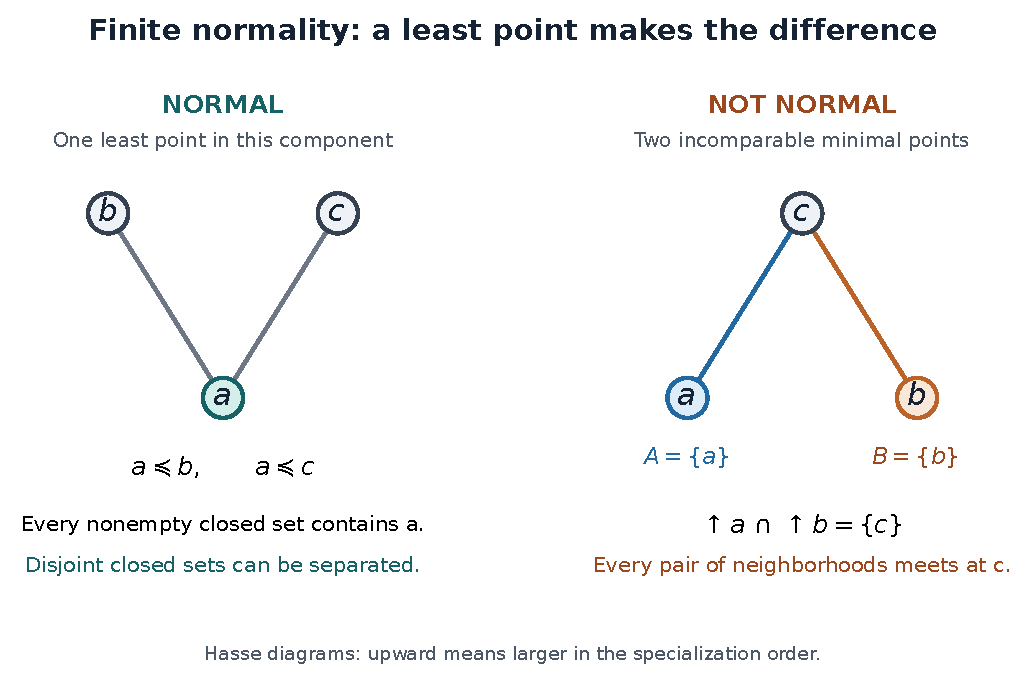
\includegraphics[width=\textwidth]{figures/finite_normality.pdf}
\caption{Open sets are upward closed. On the left, the least point $a$ lies in every nonempty closed set, so the space is normal. On the right, the disjoint closed sets $\{a\}$ and $\{b\}$ have least neighborhoods meeting at $c$; disjoint open neighborhoods and Urysohn separators do not exist.}
\label{fig:finite-normality}
\end{figure}

\subsection{Function spaces and discrete families}

\begin{theorem}[F23: finite compact-open topology and the exponential law]\label{thm:finite-exponential}
Let $C(X,Y)$ be the finite set of monotone tables between finite
spaces.  Its compact-open topology is the upward topology for
the pointwise preorder
\[
 f\preceq g\quad\Longleftrightarrow\quad
 (\forall x\in X)\ f(x)\preceq_Y g(x).
\]
Evaluation $C(X,Y)\times X\to Y$ is continuous.  For every
finite $Z$, a map $H:Z\times X\to Y$ is continuous exactly when
its curried map $z\mapsto(x\mapsto H(z,x))$ is continuous into
$C(X,Y)$.
\end{theorem}
\begin{proof}
All coded subsets $K\subseteq X$ have finite cover extraction by
F16.  The compact-open subbasic set
\[
 [K,U]=\{f:(\forall x\in K)\ f(x)\in U\}
       =\bigcap_{x\in K}[\{x\},U]
\]
is a finite intersection of point-evaluation conditions.  Each
condition is upward for pointwise order.  Conversely, the least
pointwise neighborhood of $f$ is
\[
 \mathord\uparrow f
   =\bigcap_{x\in X}[\{x\},\mathord\uparrow f(x)],
\]
which is compact-open.  Since all upward sets are unions of these
least neighborhoods, the two topologies agree.  This argument
also handles $X=\varnothing$: there is one empty map and the
empty intersection is the whole function space.

If $f\preceq g$ and $x\preceq y$, then
$f(x)\preceq g(x)\preceq g(y)$, proving evaluation monotone.
If $H$ is monotone on the product, fixing $z$ makes its section
monotone in $x$, while fixing $x$ shows pointwise monotonicity
of the curried table in $z$.  Conversely, these two monotonicity
facts give
$H(z,x)\preceq H(z',x)\preceq H(z',x')$ whenever
$(z,x)\preceq(z',x')$.  F06 translates both directions into
continuity.  Currying and uncurrying are inverse by evaluation
of their tables.  Enumerating at most $|Y|^{|X|}$ candidate
tables and testing monotonicity constructs the function-space
carrier and its pointwise relation.  Thus the proof supplies
the full finite exponential law, not only a formal analogy.
\end{proof}

\begin{theorem}[F24: finite discrete-family certificates]\label{thm:finite-discrete-family}
Given a coded indexed family $(A_i)_{i<r}$ of subsets of a finite
space, form a graph on its indices by joining distinct $i,j$
when some $x$ satisfies
\[
 \mathord\uparrow x\cap A_i\ne\varnothing,
 \qquad
 \mathord\uparrow x\cap A_j\ne\varnothing.
\]
A color class is a discrete family exactly when it contains no
graph edge.  Consequently any proper coloring supplies an
explicit decomposition into discrete families, and the greedy
algorithm always supplies at most $r$ classes.  The whole finite
family is locally finite with the uniform bound $r$.
\end{theorem}
\begin{proof}
A family is discrete when each point has an open neighborhood
meeting at most one indexed member.  Because
$\mathord\uparrow x$ is the least neighborhood of $x$, such a
neighborhood exists exactly when this least neighborhood already
meets at most one member.  Failure for a color class is exactly
an edge between two of its indices, proving the characterization.
For greedy coloring, process indices in order and choose the
least of $r$ colors absent from already colored neighbors.
At stage $i<r$ at most $i$ colors are forbidden, so a color
exists; every edge is checked when its later endpoint is colored.
Every neighborhood meets at most the $r$ indexed sets, proving
local finiteness.  Padding a finite color list by empty families
gives a certified finite instance of sigma-discreteness and
sigma-local finiteness.  No assertion about decomposing an
arbitrary infinite family follows from this finite construction.
\end{proof}

\subsection{Arithmetic proof discipline and Lean completion plan}

The algorithms above use only bounded masks, table lookup, bounded
minimum search, finite sums/products, and bounded iteration.
Their correctness proofs can be expressed with quantifier-free
Boolean invariants in \ipra.  For example, a union fold carries
the invariant that a bit is set exactly when one of the processed
sets has that bit; reachability expansion carries the invariant
that the current mask consists of vertices reachable by paths of
at most the current length.  A path code has a primitive recursive
size bound $n^{n+1}$, and removing a repeated vertex shortens its
length while preserving its endpoints.  The no-repetition
argument is finite counting on a list and is proved by bounded
induction.  A descending chain in F18 uses the same distinct-list
bound.  The elementary pigeonhole step can be verified by counting
bits, so it imports no unbounded well-foundedness principle.

For F19, use the primitive recursive predicates
$\mathrm{Preord}(n,r)$, $\mathrm{Normal}(n,r)$,
$\mathrm{Closed}(n,r,a)$, and a primitive recursive separator
constructor $s(n,r,a,b)$.  Its arithmetical assertion is
\[
\begin{split}
 &\mathrm{Preord}(n,r)\land\mathrm{Normal}(n,r)\\
 &\quad\land\mathrm{Closed}(n,r,a)\land\mathrm{Closed}(n,r,b)
 \land(a\cap b=0)\\
 &\hspace{12mm}\Longrightarrow
 \mathrm{Sep}_{01}(n,r,a,b,s(n,r,a,b)).
\end{split}
\]
Here set intersection is the bitwise primitive recursive function,
and $\mathrm{Sep}_{01}$ is the bounded test for constancy along
order pairs and for the endpoint values on the two masks.  Each
other theorem has the same shape: validity of finite input codes
implies validity of explicitly constructed output codes.  This
explains the intended first-order interpretation without claiming
that a Lean theorem about arbitrary predicates has itself already
been compiled into a checked first-order derivation.

The supplied \texttt{lean/FiniteTopology.lean} imports only
\texttt{Init}.  It defines \texttt{CPreorder}, upward and downward
predicates, interior, closure, exterior, monotone and continuous
maps, product preorders, map-space preorders, evaluation, currying,
uncurrying, and finite Boolean-table adapters.  Its checked lemmas
prove the central constructive implications in F01, F03--F04,
F06--F07, F10, and F23.  They include
\texttt{continuous\_iff\_monotone},
\texttt{closure\_idempotent},
\texttt{exterior\_iff\_not\_closure}, and the two pointwise
curry--uncurry identities.  The logged axiom audits for these
five statements report no axioms.  The file contains no admitted
proofs.  It deliberately proves the first complement identity
constructively for arbitrary predicates and leaves the converse
De Morgan identity to the decidable finite layer.

A complete formalization of this chapter has the following
concrete remaining stages.
\begin{enumerate}
\item Implement natural-number bitmask and mixed-radix encodings,
      their Boolean bounded quantifiers, and the proof that table
      decoding agrees with \texttt{Fin n} membership.  Prove the
      primitive recursive defining equations in the chosen
      ProveIt arithmetic syntax.
\item Formalize binary-fold topology tables, prove F02 by the
      explicit minimal-neighborhood construction, and specialize
      the checked order-theoretic kernel to these tables.
\item Implement Warshall closure and component expansion with the
      bounded path invariants stated above.  Use these to prove
      F11--F14 and the canonical $T_0$ quotient.
\item Prove the finite distinct-list bound and the normality
      characterization F18.  The Boolean separator in F19 and
      rational table extension in F20 then follow by component
      constancy.  These are genuine remaining proof obligations,
      not axioms supplied to make an endpoint type-check.
\item Check the rational metric tables and function-space
      enumerator, and transport the already checked evaluation
      and currying lemmas to the encoded carrier.  Finish the
      discrete-family graph criterion and bounded coloring proof.
\item Compile the resulting finite invariant proofs into explicit
      \ipra\ derivations, and run the object-theory proof checker.
      Until this final step is implemented, the artifact is a
      checked Lean kernel plus a detailed \ipra\ proof plan, not
      a completed kernel-checked formalization in the object theory.
\end{enumerate}

The independent standard-library Python checker exhaustively
examines all preorders on carriers of size $0$ through $4$;
their counts are $1,1,4,29,355$.  It independently enumerates
topology tables through size $3$, checks $92\,805$
closure/interior pairs, $24\,907$ map tables, $391$ quotient
instances, and $36$ compact-open exponentials.  It also checks
$4\,133$ two-valued separators and $7\,688$ rational-valued
extension instances (using the value alphabet $\{0,1,2\}$).
The exact results are in \texttt{data/finite\_coverage.json}.
These finite checks catch orientation, coding, and statement errors;
the uniform mathematical justification is the proofs above.

\section{Metric topology with explicit computational data}
\label{sec:metric}

\subsection{What the metric replacements assert}

The four entries treated here are Tychonoff's theorem,\footnote{\url{https://mathworld.wolfram.com/TychonoffTheorem.html}}
Urysohn's lemma,\footnote{\url{https://mathworld.wolfram.com/UrysohnsLemma.html}}
Urysohn's metrization theorem,\footnote{\url{https://mathworld.wolfram.com/UrysohnsMetrizationTheorem.html}}
and the compact-open topology.\footnote{\url{https://mathworld.wolfram.com/Compact-OpenTopology.html}}  They concern
infinite objects in their usual formulations.  The replacements below are
families of arithmetic assertions about names, moduli, finite nets, and
finite computations.  The displayed real-valued notation is an explanatory
interpretation of those assertions; it does not add a sort of arbitrary
real numbers or arbitrary subsets to \ipra.

A named real is given by a fixed primitive-recursive rational approximation
procedure with its error estimate.  We write $q(k)\simeq_k r$ for
$|q(k)-r|\leq 2^{-k}$.  A named point has enough data to compute the
rational approximations of the distances used below.  All operations are
understood in a fixed, explicitly given primitive-recursive presentation.
When a family of spaces is indexed by $i$, the procedures involving $i$
must be uniformly primitive recursive.  The phrase ``given a procedure''
means a particular function symbol with its defining equations and the
stated hypotheses, or a proof schema after substituting that procedure.
It never means that arbitrary primitive-recursive program codes can be
uniformly evaluated by another primitive-recursive program.

For a metric space $X$, the following data have different roles.
\begin{itemize}
\item A modulus for a map $f:X\to Y$ is a function $\mu$ satisfying
\begin{equation}\label{eq:metric-modulus}
d_X(x,y)\leq 2^{-\mu(k)}\quad\Longrightarrow\quad
 d_Y(f(x),f(y))\leq 2^{-k}.
\end{equation}
Replacing $\mu(k)$ by $\max_{j\leq k}\mu(j)$ makes it monotone.
\item A net is a finite list $P_k=(p_{k,j})_{j<M(k)}$ together with a
selector $\sigma_k(x)<M(k)$ and a proof of
$d_X(x,p_{k,\sigma_k(x)})\leq 2^{-k}$.  The selector is useful data;
it is not obtained by deciding inequalities between arbitrary reals.
\item A Cauchy modulus for a sequence $(x_n)$ is a function $m$ such that
$n,l\geq m(k)$ implies $d_X(x_n,x_l)\leq 2^{-k}$.
\item A completion operation, when assumed, takes the particular supplied
Cauchy data to a point name and a convergence modulus.  The existence of
an arbitrary limit is not being used as a choice principle.
\end{itemize}
Distances can be truncated at $1$ without changing the metric topology:
$\bar d=\min(1,d)$ is a metric because
$\min(1,a+b)\leq\min(1,a)+\min(1,b)$.  The triangle inequality for
$\bar d$ follows immediately.  The balls of radius less than $1$ coincide
with the corresponding $d$-balls.  Finite minima and maxima of named reals
are computed by $\max(a,b)=(a+b+|a-b|)/2$, so their use does not invoke
real-order decidability.

\begin{remark}[Finite-demand meaning]\label{rem:metric-finite-demand}
Every precision-$k$ conclusion below depends on explicitly bounded lists,
finite sums, and rational inequalities.  Rational inequalities are tested
by cross multiplication with positive denominators.  A proof can replace
all finite bounded quantifiers by their primitive-recursive Boolean folds.
The correctness invariant for the relevant loop is then quantifier free
with the input codes as parameters.  Analytic notation abbreviates these
uniform estimates, not an unproved global soundness theorem for all such
notations.  The Lean file supplied with this chapter checks some abstract
metric-interface lemmas and states the remaining implementation targets;
it is not a derivation of every displayed theorem inside an encoded
\ipra\ proof calculus.
\end{remark}

\subsection{Products: a constructive Tychonoff replacement}

\begin{theorem}[Finite products of explicit nets]\label{thm:finite-metric-product}
Let $X_0,\ldots,X_{r-1}$ have nets at every precision, and equip their
product with $d_{\max}(x,y)=\max_{i<r}d_i(x_i,y_i)$.  The Cartesian
product of the precision-$k$ nets is a precision-$k$ net, of size
$\prod_{i<r}M_i(k)$.  Its selector and list are primitive recursive.
For $r=0$ the product consists of one empty tuple.
\end{theorem}
\begin{proof}
For each coordinate choose the supplied index $\sigma_{i,k}(x_i)$.
Every coordinate distance to the resulting tuple is at most $2^{-k}$,
so their maximum is at most $2^{-k}$.  Mixed-radix enumeration of the
finite tuple of indices gives both the list and the selected index.
Only bounded products and bounded loops are used.  If a factor is empty,
there is no input product point to select; its empty net is appropriate.
\end{proof}

For a countable family assume bounded metrics $0\leq d_i\leq 1$ and
specified base points $p_i$.  A product point is a uniformly presented
family $(x_i)$, not an arbitrary externally chosen sequence.  Define
\begin{equation}\label{eq:product-metric}
 D(x,y)=\sum_{i=0}^{\infty}2^{-i-1}d_i(x_i,y_i),\qquad
 D_N(x,y)=\sum_{i<N}2^{-i-1}d_i(x_i,y_i).
\end{equation}
The sum is shorthand for a name with the certified bound
\begin{equation}\label{eq:product-tail}
0\leq D(x,y)-D_N(x,y)\leq 2^{-N}.
\end{equation}

\begin{theorem}[Weighted product metric and its neighborhoods]
\label{thm:weighted-product}
The procedure in \eqref{eq:product-metric} defines a named metric.
It satisfies
\begin{equation}\label{eq:coordinate-bound}
 2^{-i-1}d_i(x_i,y_i)\leq D(x,y).
\end{equation}
Its neighborhoods agree with the finite-coordinate product neighborhoods,
with explicit transformations in both directions.
\end{theorem}
\begin{proof}
The finite geometric sum gives
$\sum_{i=N}^{L-1}2^{-i-1}\leq 2^{-N}$ for every $L\geq N$;
this proves the Cauchy estimate defining the sum.  For a precision-$k$
name, sum the first $k+2$ terms using distance approximations of error
$2^{-k-2}$.  Their weighted error is at most $2^{-k-2}$, and the omitted
tail has the same bound.  Thus the total error is at most $2^{-k-1}$.
Nonnegativity, symmetry, and the triangle inequality hold first for finite
sums and then at every demanded precision.  If $D(x,y)=0$, the nonnegative
summand bound gives $d_i(x_i,y_i)=0$ for every fixed $i$, hence coordinate
identity.  No decision between equality and inequality is involved.

For a finite cylinder requiring $d_i(x_i,y_i)<r_i$ for $i<N$, the positive
rational radius
$\rho=\min_{i<N}2^{-i-1}r_i$ satisfies
$D(x,y)<\rho\Rightarrow d_i(x_i,y_i)<r_i$ for all its coordinates.
The empty cylinder is the whole space.  Conversely, to obtain
$D(x,y)<2^{-k}$, put $N=k+2$ and require
$d_i(x_i,y_i)<2^{-k-2}$ for $i<N$.  The partial sum is less than
$2^{-k-2}$ and the tail is at most $2^{-k-2}$; their sum is less than
$2^{-k-1}<2^{-k}$.  General positive rational radii are reduced to dyadic
ones by a bounded calculation on their numerator and denominator.
\end{proof}

\begin{theorem}[Countable products of explicit nets]
\label{thm:countable-net-product}
Suppose the base points, nets, and selectors are supplied uniformly in
$i$.  The product has a primitive-recursive net of size
\begin{equation}\label{eq:product-net-size}
 M(k)=\prod_{i<k+2}M_i(k+2).
\end{equation}
A net point uses a net coordinate in positions $i<k+2$ and the fixed base
point $p_i$ in every remaining position.  Its distance from the selected
input point is at most $2^{-k-1}$.
\end{theorem}
\begin{proof}
For the first $k+2$ coordinates the error is at most $2^{-k-2}$.
Their weighted contribution is at most that quantity.  The unused tail
is at most $2^{-k-2}$.  Sum these bounds.  Listing and selecting the finite
coordinate tuple uses the algorithm of
Theorem~\ref{thm:finite-metric-product}; evaluating its other coordinates
uses the given base-point procedure.  In particular, no countable choice
of points in unspecified nonempty factors occurs.
\end{proof}

\begin{theorem}[Transport of supplied completion procedures]
\label{thm:product-completion}
Suppose coordinate completion is available uniformly: from the specific
coordinate Cauchy data it produces a name $z_i$ and a convergence modulus
$c_i$.  Then completion of the corresponding product sequence is
primitive recursive.  A valid product convergence modulus is
\begin{equation}\label{eq:product-completion-rate}
 c(k)=\max_{i<k+2}c_i(k+2).
\end{equation}
Product Cauchy data with modulus $m$ furnish coordinate-$i$ Cauchy data
with modulus $k\mapsto m(k+i+1)$.
\end{theorem}
\begin{proof}
The second assertion follows from
$d_i\leq 2^{i+1}D$.  Apply the given coordinate completion procedure to
these data, uniformly in $i$.  If $n\geq c(k)$, each of the first $k+2$
coordinate distances from $z_i$ is at most $2^{-k-2}$.  The same
partial-sum and tail estimate used for the net gives
$D(x_n,z)\leq 2^{-k-1}$.  Each finite request to the product name makes
only finitely many calls to the supplied uniform procedure.
\end{proof}

Theorems~\ref{thm:countable-net-product} and
\ref{thm:product-completion} are a useful version of countable product
compactness when compactness is represented by completeness data and
finite nets.  They do not assert the open-cover compactness of an
arbitrary product or extract a modulus from an arbitrary cover.
The distinction is essential: the MathWorld Tychonoff entry discusses an
arbitrary family, and explicitly records its relation to choice.
There is also a classical edge case in the entry's opening ``if and only
if'': an empty product space may be compact even if one of its other
factors is noncompact.  The converse from compact product to compact
factors requires a nonempty product, for example specified base points.

\begin{proposition}[Uniform images preserve nets]\label{prop:image-nets}
If $f$ has modulus $\mu$ and $P_k$ is a net for $X$, then
$(f(p))_{p\in P_{\mu(k)}}$ covers the represented image of $f$ at
precision $k$, with a selector supplied by the preimage presentation.
\end{proposition}
\begin{proof}
For an image point presented as $f(x)$, use
$f(p_{\mu(k),\sigma_{\mu(k)}(x)})$ and apply
\eqref{eq:metric-modulus}.  This does not choose a preimage from a bare
extensional membership assertion.  Completeness of an image is not
claimed merely from this net calculation.
\end{proof}

\subsection{Urysohn functions from located distance data}

A distance function to a general closed set need not be computable from
a negative description of that set.  We therefore include the functions
needed for the construction in the input.  Let $a,b:X\to[0,\infty)$ be
supplied $1$-Lipschitz named functions, with $a=0$ on $A$ and $b=0$ on
$B$.  They may be the located distances to $A$ and $B$.

\begin{theorem}[Urysohn separation with a positive gap]
\label{thm:metric-urysohn}
If $a(x)+b(x)\geq\delta>0$ for all $x$, where $\delta$ is a positive
rational input, then
\begin{equation}\label{eq:urysohn-function}
 u(x)=\frac{a(x)}{a(x)+b(x)}
\end{equation}
is a named function with values in $[0,1]$, is $1/\delta$-Lipschitz,
and equals $0$ on $A$ and $1$ on $B$.  Its approximation procedure and
modulus are primitive recursive in the supplied data.
\end{theorem}
\begin{proof}
Write $a=a(x)$, $b=b(x)$, $a'=a(y)$, $b'=b(y)$, and $s=a+b$,
$s'=a'+b'$.  The denominator is positive and
\[
 \left|\frac{a}{s}-\frac{a'}{s'}\right|
 =\frac{|ab'-a'b|}{ss'}
 \leq\frac{a|b'-b|+b|a-a'|}{ss'}
 \leq\frac{d(x,y)}{s'}\leq\frac{d(x,y)}{\delta}.
\]
This proof gives the sharper constant $1/\delta$, with no factor of $2$.
The interval bound follows from $0\leq a\leq s$.  On $A$ the numerator
vanishes, while on $B$ one has $s=a\geq\delta$.

For computation approximate $a,b$ with error $\eta$ and clamp the
approximations to be nonnegative.  Clamping cannot increase the error.
If $2\eta\leq\delta/2$, their approximate sum $\widehat s$ is at least
$\delta/2$.  The same numerator calculation gives
\[
 \left|\frac{a}{s}-\frac{\widehat a}{\widehat s}\right|
 \leq\frac{\eta}{\widehat s}\leq\frac{2\eta}{\delta}.
\]
Choose a natural number $h$ with
$2^{-h}\leq\min(1,\delta)/8$, and evaluate at precision $k+h$.
The error is at most $2^{-k-2}$.  Such an $h$ can be obtained by a
bounded search using the denominator of the positive rational $\delta$.
A uniform-continuity modulus is obtained by choosing $\mu(k)$ so that
$2^{-\mu(k)}\leq\delta 2^{-k}$.  Every division is by an explicitly
positive rational approximation.
\end{proof}

\begin{proposition}[Local-gap Urysohn separation]
\label{prop:local-urysohn}
A global lower bound is unnecessary for pointwise continuity.  It is
enough to supply, for every presented $x$, a positive rational
$\delta_x\leq a(x)+b(x)$, by a primitive-recursive procedure.  Formula
\eqref{eq:urysohn-function} then has a computable local modulus: if
$d(x,y)\leq\delta_x/4$, then
\[
 |u(x)-u(y)|\leq 2d(x,y)/\delta_x.
\]
\end{proposition}
\begin{proof}
Since $a+b$ is $2$-Lipschitz,
$a(y)+b(y)\geq\delta_x-2d(x,y)\geq\delta_x/2$.
Use the numerator estimate from the preceding proof with this denominator.
Evaluation at $x$ uses $\delta_x$ exactly as in that proof.  Thus a
local modulus may demand simultaneously
$d(x,y)\leq\delta_x/4$ and
$d(x,y)\leq\delta_x 2^{-k-1}$.
Disjointness alone does not supply the distance functions or this local
lower-bound procedure.
\end{proof}

\begin{corollary}[Finite rational metric sets]
\label{cor:finite-metric-urysohn}
Let $A,B$ be nonempty disjoint finite subsets of a rational metric space,
and suppose their displayed points are pairwise distinguishable by the
metric.  Put
\[
 a(x)=\min_{p\in A}d(x,p),\quad b(x)=\min_{q\in B}d(x,q),\quad
 \delta=\min_{p\in A,q\in B}d(p,q)>0.
\]
The data satisfy Theorem~\ref{thm:metric-urysohn}.
\end{corollary}
\begin{proof}
Each distance-to-a-point function is $1$-Lipschitz; taking a finite minimum
preserves that bound.  A rational finite minimum attains its value by
bounded comparison.  At minimizing $p,q$, the triangle inequality gives
$\delta\leq d(p,q)\leq d(p,x)+d(x,q)=a(x)+b(x)$.
Finite disjointness and positivity of rational nonzero distances make
the displayed minimum positive.  All lists and comparisons are bounded.
If one of the sets is empty, a constant function supplies the required
nonempty-side boundary value instead.
\end{proof}

\subsection{Metrization by separating coordinates}

The existence of many separating functions does not by itself provide
a computable inverse for the map they define.  The following formulation
records exactly the extra local information that is used.

\begin{theorem}[Coordinate metrization with a neighborhood certificate]
\label{thm:coordinate-metrization}
Let $X$ have a represented neighborhood basis.  Suppose a uniformly
presented family $u_i:X\to[0,1]$ is given with local continuity moduli.
Assume two further pieces of data.
\begin{enumerate}
\item Coordinate equality identifies points: if $u_i(x)=u_i(y)$ for
all $i$, then $x=y$ in the chosen representation.
\item Given a certified basic neighborhood $V$ of $x$, a procedure returns
$N$ and a positive rational $\varepsilon$ such that
\[
 (\forall i<N)\ |u_i(x)-u_i(y)|<\varepsilon\quad\Longrightarrow\quad y\in V.
\]
\end{enumerate}
Then
\[
 d_u(x,y)=\sum_{i\geq0}2^{-i-1}|u_i(x)-u_i(y)|
\]
is a compatible named metric, and $x\mapsto(u_i(x))_i$ is a homeomorphism
onto its represented image in the Hilbert cube.  The inverse
neighborhood transformation can use radius $2^{-N}\varepsilon$.
\end{theorem}
\begin{proof}
The metric axioms and computation follow from
Theorem~\ref{thm:weighted-product}.  Its zero-distance implication is the
first hypothesis.  For continuity at precision $k$, use $N=k+2$ and
intersect the finitely many neighborhoods on which the first $N$
coordinates change by less than $2^{-k-2}$.  The finite sum and tail
give a change less than $2^{-k}$.  The finite intersection and its
refinement are part of the presented basis operations.

Conversely, if $d_u(x,y)<2^{-N}\varepsilon$, then for $i<N$,
\[
 |u_i(x)-u_i(y)|\leq 2^{i+1}d_u(x,y)
 <2^{i+1-N}\varepsilon\leq\varepsilon.
\]
The second hypothesis now gives $y\in V$.  Both neighborhood transformations
are explicit finite calculations.  An inverse is considered only on the
represented image, whose points carry an $X$-name; no algorithm extracting
an arbitrary preimage is implicit.
\end{proof}

This theorem isolates a constructive part of Urysohn's metrization proof.
It does not produce the coordinate functions and their neighborhood
certificates from bare regularity and a bare countable basis.  Those are
additional proof obligations for a particular presentation.

\begin{theorem}[An explicit Hilbert-cube embedding for a separable metric
presentation]\label{thm:dense-hilbert-embedding}
Let $X$ have a specified dense sequence $(p_i)$ and a primitive-recursive
locator $\lambda(x,k)$ satisfying
$d(x,p_{\lambda(x,k)})\leq2^{-k}$.  Define
\[
 u_i(x)=\min(1,d(x,p_i)),\qquad E(x)=(u_i(x))_{i\geq0}.
\]
Then $E$ is an embedding into the Hilbert cube.  Its forward map is
$1$-Lipschitz for the weighted metric, and an explicit inverse local
modulus is
\begin{equation}\label{eq:dense-embedding-inverse}
 D(E(x),E(y))<2^{-(\lambda(x,k+2)+k+2)}
 \quad\Longrightarrow\quad d(x,y)<2^{-k}.
\end{equation}
\end{theorem}
\begin{proof}
Truncation and the reverse triangle inequality give
$|u_i(x)-u_i(y)|\leq\min(1,d(x,y))$; summing the weights gives
$D(E(x),E(y))\leq d(x,y)$.  Put $r=2^{-k}\leq1$ and
$i=\lambda(x,k+2)$.  The hypothesis of
\eqref{eq:dense-embedding-inverse} and the coordinate bound imply
$|u_i(x)-u_i(y)|<r/2$.  Since $u_i(x)\leq r/4$,
$u_i(y)<3r/4<1$.  Thus the truncation is inactive at $y$, and
\[
 d(x,y)\leq d(x,p_i)+d(p_i,y)<r/4+3r/4=r.
\]
This also proves that coordinate equality forces point equality.  Every
index and requested precision in this argument is explicitly computable.
The inverse modulus depends on $x$; no uniform bound on the locator's
index is asserted.
\end{proof}

\subsection{Euclidean examples and explicit homeomorphisms}

The Euclidean-topology and homeomorphism entries supply the classical
terminology for the following concrete constructions.\footnote{\url{https://mathworld.wolfram.com/EuclideanTopology.html};
\url{https://mathworld.wolfram.com/Homeomorphism.html}}

\begin{proposition}[Euclidean norm comparisons]
\label{prop:euclidean-norms}
For $v\in\R^d$, with $d\geq1$,
\[
 \|v\|_\infty\leq\|v\|_2\leq\|v\|_1
 \leq d\|v\|_\infty.
\]
Consequently these metrics induce the same topology by explicit rational
moduli.  Rational grids give nets for bounded rational boxes, and rational
vectors give a dense sequence with a locator for represented points.
\end{proposition}
\begin{proof}
Each $v_i^2$ is at most $\sum_jv_j^2$, so
$|v_i|\leq\|v\|_2$.  Expanding
$(\sum_i|v_i|)^2$ gives $\sum_iv_i^2$ plus nonnegative cross terms,
which proves the middle inequality.  The last inequality sums
$|v_i|\leq\|v\|_\infty$.  Squaring reduces the only square-root
comparisons to rational inequalities with nonnegative sides; the
nonnegative square root has its usual bisection name on a supplied bounded
interval.  For a requested Euclidean error $2^{-k}$, choose a grid of
sup-norm mesh at most $2^{-k}/d$.  Clamping coordinate approximations
to a bounded box preserves the required bounds.  Finite products enumerate
the grid, and standard rational-tuple coding enumerates the dense sequence.
The grid selector uses rational approximations with extra slack, not exact
comparison of a real coordinate with a grid boundary.
\end{proof}

\begin{proposition}[A named homeomorphism between Euclidean space and an
open cube]\label{prop:euclidean-open-cube}
Coordinatewise application of
\[
 h(t)=\frac{t}{1+|t|},\qquad h^{-1}(s)=\frac{s}{1-|s|}
\]
gives a homeomorphism $\R^d\cong(-1,1)^d$.  The forward map is
$1$-Lipschitz in sup norm.  On the subcube $|s_i|\leq1-\delta$,
$\delta>0$, the inverse is $\delta^{-2}$-Lipschitz.
\end{proposition}
\begin{proof}
The two formulas are inverse by elementary substitution, separately on
the nonnegative and nonpositive rational approximations, or directly
using the identities for absolute value.  For two real numbers of the
same sign,
\[
 |h(t)-h(u)|=\frac{|t-u|}{(1+|t|)(1+|u|)}\leq|t-u|.
\]
For opposite signs, $|h(t)-h(u)|=|h(t)|+|h(u)|\leq|t|+|u|=|t-u|$.
The inverse calculation on a same-sign interval has denominator
$(1-|s|)(1-|v|)\geq\delta^2$; across zero use the sum of the two
one-sided estimates.  These inequalities can also be proved by rational
case splits followed by approximation, so they require no trichotomy for
arbitrary named reals.  Evaluation of the inverse at an open-cube point
uses a supplied positive distance from each coordinate to the endpoints.
Taking a finite minimum of those distances supplies $\delta$.
\end{proof}

\subsection{Function spaces and the compact-open topology}

Let $K$ be an inhabited represented metric space equipped with nets.
For maps $f,g:K\to Y$ with supplied moduli, the function
$h(x)=d_Y(f(x),g(x))$ has modulus
\begin{equation}\label{eq:distance-function-modulus}
 \nu(k)=\max\{\mu_f(k+1),\mu_g(k+1)\}.
\end{equation}
Indeed, the reverse triangle inequality gives
$|h(x)-h(y)|\leq d(f(x),f(y))+d(g(x),g(y))$.

\begin{theorem}[Computable uniform metric]
\label{thm:computable-uniform-metric}
With the above data, the quantity
\[
 d_\infty(f,g)=\sup_{x\in K}d_Y(f(x),g(x))
\]
has a primitive-recursive real name.  It is obtained from finite maxima
on nets, and is a metric on maps identified pointwise.  No exact
maximizing point is required.
\end{theorem}
\begin{proof}
At precision $k$ put $\eta=2^{-k-3}$ and take a net at
precision $\nu(k+3)$.  Approximate each of the finitely many values
$h(p_j)$ by $q_j$ with error at most $\eta$, and let $Q_k=\max_jq_j$,
using ordinary rational comparisons.  For every $x$, the selected net
point gives
\[
 h(x)\leq h(p_{\sigma(x)})+\eta\leq Q_k+2\eta.
\]
For a rational maximizing index $j_k$,
$h(p_{j_k})\geq Q_k-\eta$.  Thus $[Q_k-\eta,Q_k+2\eta]$ is a
certified interval for the supremum.  Any two such intervals are
compatible: each upper endpoint bounds every actual value, including the
net value witnessing the other's lower endpoint.  Consequently the
$Q_k$ form a Cauchy name with the displayed error bounds, defining a real
$S$ satisfying $h(x)\leq S$ for every $x$ and
$S\leq Q_k+2\eta$.  If $b$ bounds every $h(x)$ then
$Q_k\leq b+\eta$ for every $k$, hence $S\leq b$ at all precisions.
This proves the claimed supremum property without assuming a general
least-upper-bound axiom.

Symmetry and nonnegativity are inherited pointwise.  For every $x$,
$d(f(x),h(x))\leq d(f(x),g(x))+d(g(x),h(x))$; taking the certified
upper bounds gives the triangle inequality.  If $d_\infty(f,g)=0$,
every pointwise distance is zero, so the maps agree in the chosen
pointwise equivalence.  Every computation made at precision $k$ is a
finite maximum on an explicitly sized net.
\end{proof}

\begin{corollary}[Approximate extrema]
\label{cor:approximate-extrema}
For a real-valued uniformly continuous function $v$ on a represented
inhabited space with nets, a primitive-recursive procedure returns
$x_k\in K$ with
\[
 (\forall x\in K)\quad v(x)\leq v(x_k)+2^{-k}.
\]
An analogous procedure gives an approximate minimum.
\end{corollary}
\begin{proof}
Take a net fine enough that the variation of $v$ between a point and its
selected net point is at most $\eta=2^{-k-2}$.  Approximate the net
values with error at most $\eta$ and choose a largest rational
approximation, at $x_k$.  For every $x$,
\[
 v(x)\leq v(p_{\sigma(x)})+\eta
 \leq q_{\sigma(x)}+2\eta
 \leq q_{x_k}+2\eta
 \leq v(x_k)+3\eta<v(x_k)+2^{-k}.
\]
Apply the same algorithm to $-v$ for minima.  An exact maximizer or a
convergent subsequence of maximizing points is a different assertion and
is not extracted here.
\end{proof}

For the next result take $K=[0,1]^d$ with the sup metric and its usual
dyadic box data.  Write
\[
 [C,U]=\{g:g(C)\subseteq U\}
\]
for a compact-open subbasic condition.  The closed dyadic boxes used
below have explicit product nets and completion procedures.  Thus the
word ``compact'' here comes with the data already constructed, and not
with a universal open-cover elimination principle.

\begin{theorem}[An explicit compact-open neighborhood comparison on a
cube]\label{thm:compact-open-cube}
Let $f:[0,1]^d\to Y$ have a supplied uniform modulus and let
$\varepsilon>0$ be rational.  A primitive-recursive procedure constructs
finitely many closed dyadic boxes $C_j$ covering the cube, points
$p_j\in C_j$, and balls
$U_j=B(f(p_j),\varepsilon/2)$ such that
\begin{equation}\label{eq:compact-open-sandwich}
 B_{\infty}(f,\varepsilon/4)
 \ \subseteq\ \bigcap_j[C_j,U_j]
 \ \subseteq\ B_{\infty}(f,\varepsilon).
\end{equation}
In particular these finitely certified compact-open neighborhoods
and the uniform metric generate the same local neighborhoods for the
represented maps in question.
\end{theorem}
\begin{proof}
Choose a dyadic step $h=2^{-N}$ fine enough that the modulus guarantees
$d_Y(f(x),f(p))\leq\varepsilon/4$ whenever
$\|x-p\|_\infty\leq h$.  Enumerate the grid centers $p_j$ with
coordinates in $\{0,h,2h,\ldots,1\}$ and set
$C_j=\prod_i[\max(0,p_{j,i}-h),\min(1,p_{j,i}+h)]$.
These boxes overlap.  To cover a named point $x$, approximate each
coordinate within $h/4$, clamp the rational approximation to $[0,1]$,
and round it to a nearest grid value.  The resulting center has distance
at most $3h/4$ from $x$, so it selects a containing box with slack.
Enumeration, rational rounding, and the required mesh exponent are
primitive recursive.

If $d_\infty(f,g)<\varepsilon/4$, then for $x\in C_j$,
\[
 d(g(x),f(p_j))
 \leq d(g(x),f(x))+d(f(x),f(p_j))<\varepsilon/2.
\]
This proves the first inclusion.  If $g$ lies in all the displayed
subbasic conditions, select any box containing $x$; then
\[
 d(f(x),g(x))<\varepsilon/4+\varepsilon/2=3\varepsilon/4.
\]
Taking the supremum gives $d_\infty(f,g)\leq3\varepsilon/4<\varepsilon$,
which proves the second inclusion with a uniform positive margin.
The overlap matters constructively: an exact partition into adjacent
closed boxes would ask for a side decision at an arbitrary real boundary.
Our rational-approximation selector makes no such decision.
\end{proof}

For a general compact-open condition $[C,U]$, the analogous finite-demand
statement assumes a supplied margin $\delta>0$ such that
$B(f(x),\delta)\subseteq U$ for all $x\in C$.  Then
$B_\infty(f,\delta)\subseteq[C,U]$ by direct substitution.
No procedure obtaining such a margin from a bare assertion
$f(C)\subseteq U$ has been claimed.  This is the precise limitation of
the comparison with the unrestricted compact-open theorem.

\begin{proposition}[Evaluation with an explicit local modulus]
\label{prop:metric-evaluation}
For modulus-equipped maps on $K$, evaluation $(f,x)\mapsto f(x)$ is
continuous in the uniform metric.  At $(f,x)$, it is enough to require
\[
 d_\infty(f,g)\leq2^{-k-1},\qquad
 d_K(x,y)\leq2^{-\mu_f(k+1)}
\]
to obtain $d_Y(f(x),g(y))\leq2^{-k}$.
\end{proposition}
\begin{proof}
Insert $f(y)$ and use the triangle inequality:
$d(f(x),g(y))\leq d(f(x),f(y))+d(f(y),g(y))
\leq2^{-k-1}+2^{-k-1}$.
The dependence of this local modulus on $f$ is explicit.
\end{proof}

\begin{theorem}[A quantitative exponential-law fragment]
\label{thm:metric-currying}
Suppose $H:K\times Z\to Y$ has a supplied uniform modulus $\mu$ for
the maximum product metric.  Then its curry
$\widehat H(z)(x)=H(x,z)$ has the same modulus as a map to the uniform
metric on $C(K,Y)$.  Conversely, suppose the curry has a modulus
$\alpha$, and all its slices have a common modulus $\beta$ in $x$.
Then $H$ has modulus
\[
 \gamma(k)=\max\{\alpha(k+1),\beta(k+1)\}.
\]
\end{theorem}
\begin{proof}
If $d_Z(z,z')\leq2^{-\mu(k)}$, apply uniform continuity of $H$ to
$(x,z),(x,z')$ for every $x$.  The supremum of their distances is at most
$2^{-k}$.  In the converse direction insert $H(x,z')$:
\[
 d(H(x,z),H(x',z'))
 \leq d(H(x,z),H(x,z'))+d(H(x,z'),H(x',z'))
 \leq2^{-k-1}+2^{-k-1}.
\]
The first term is bounded by the uniform metric between the slices and
the second by their common modulus.  This is a quantitative statement
with supplied uniformity; it is not a derivation of the unrestricted
locally-compact Hausdorff exponential law from bare continuity.
\end{proof}

\subsection{Arithmetic and Lean implementation route}

The finite sum identity behind \eqref{eq:product-tail}, mixed-radix tuple
enumeration, finite maxima, and rational cross-multiplication are the
arithmetic core.  A direct implementation has the following layers.
\begin{enumerate}
\item Encode integers, positive-denominator rationals, lists, tuples, and
finite tables by natural numbers.  Define rational comparison by the
integer cross products, and define every list fold by primitive recursion.
\item Implement each fixed approximation, net, selector, and modulus
procedure as primitive-recursive syntax.  Prove the finite numerical
invariant of each loop by quantifier-free induction.  Rational arithmetic
identities can be proved in the standard definitional extension for
primitive-recursive functions and translated to the selected presentation
of \ipra.
\item Represent a real equation or inequality by its finite precision
tests.  Division carries a positive-denominator certificate; suprema and
infinite sums carry the explicit Cauchy bounds proved above.  The
product construction requests at most $k+2$ coordinates for a
precision-$k$ output.  The embedding requests the one locator index
shown in \eqref{eq:dense-embedding-inverse}.
\item In Lean, first formalize these finite rational statements, then
prove the representation theorems interpreting them as the usual metric
claims.  The supplied \texttt{MetricBlueprint.lean} checks the basic
precision-space product and modulus-composition arguments without
\texttt{sorry}.  Its semantic function fields are interfaces, not claims
that all Lean functions are primitive recursive.
\item For an actual internal endpoint, compile the selected algorithms
and proof invariants into the repository's object-language syntax and
produce its proof predicate.  This last compilation is an explicitly
remaining formalization task; Lean's ordinary kernel checking of an
external semantic theorem does not perform it automatically.
\end{enumerate}
These steps distinguish useful fully proved constructive mathematical
reductions from an assertion that the entire classical topology library
has already been formalized inside \ipra.

\section{Finite algebraic topology, sheaves, and Boolean algebras}
\label{sec:algebraic}

This section treats the index entries \emph{Betti Number}, \emph{Euler
Characteristic}, \emph{Genus}, \emph{Coloring}, the sheaf-related entries, and
\emph{Sigma-Algebra}.  The objects are finite tables or finite presentations.
Consequently the results below are uniform arithmetic theorems about those
presentations, not assertions that an arbitrary topological space has a
finite presentation.  The distinction matters especially for homotopy
invariance, surface classification, and countable unions.

\subsection{Chain complexes and exact computation of homology}

A finite rational chain complex consists of a natural number $d$, dimensions
$c_0,\ldots,c_d$, and rational matrices
\[
 D_k:\Q^{c_k}\longrightarrow\Q^{c_{k-1}}
 \qquad(1\leq k\leq d)
\]
whose consecutive products vanish.  Put $c_{-1}=c_{d+1}=0$ and let $D_0$ and
$D_{d+1}$ be the zero maps to and from the zero-dimensional spaces.  A matrix
is a rectangular list; a rational entry is an integer numerator and a
positive integer denominator.  All equalities in this subsection are
checked by cross multiplication.  In particular, no equality test for real
numbers occurs.  Write
\[
 Z_k=\ker D_k,\qquad B_k=\operatorname{im}D_{k+1},\qquad
 H_k=Z_k/B_k.
\]
The quotient notation will be implemented by a chosen basis and a projection,
as described below, rather than by a primitive quotient sort.

\begin{proposition}[A01: the simplicial boundary squares to zero]
\label{prop:boundary-square}
Let $K$ be a finite list of nonempty increasing vertex lists, closed under
nonempty sublists.  For $k>0$ define
\[
 \partial[v_0,\ldots,v_k]
   =\sum_{i=0}^{k}(-1)^i[v_0,\ldots,\widehat v_i,\ldots,v_k],
 \qquad \partial[v]=0.
\]
The resulting integer matrices satisfy $\partial^2=0$.
\end{proposition}
\begin{proof}
Fix two distinct deleted vertices with original indices $i<j$.  Deleting
$j$ first and then $i$ contributes sign $(-1)^{i+j}$ to the remaining
face.  Deleting $i$ first and then the vertex now in position $j-1$
contributes $(-1)^{i+j-1}$.  These contributions cancel.  Every term in the
double sum belongs to exactly this pair, indexed by $i<j$.  For $k=1$ the
second boundary is zero by definition.  This is a finite reindexing of
integer sums, formalizable by bounded induction on the two indices.
\end{proof}

\begin{proposition}[A02: homology with explicit normal forms]
\label{prop:effective-homology}
There is a primitive recursive algorithm computing integers $r_k$ and
$b_k$, rational matrices giving cycle and boundary bases, and mutually inverse
coordinate maps
\[
 H_k\cong\Q^{b_k},\qquad
 r_k=\operatorname{rank}D_k,\qquad
 b_k=c_k-r_k-r_{k+1}.
\]
In particular $r_k+r_{k+1}\leq c_k$.
\end{proposition}
\begin{proof}
Process the columns of a matrix from left to right.  At each step scan the
unused rows in their fixed order; if a nonzero entry exists, choose the first
one, exchange rows, divide the pivot row by that entry, and subtract its
appropriate multiples from every other row.  If there is no such entry,
move to the next column.  The procedure performs at most the number of
columns many stages, each with a bounded row scan.  Every row operation has
an explicitly recorded inverse.  The final reduced matrix therefore has
the same kernel as the original matrix and has $r$ pivot columns.  Its
nonpivot variables are free; assigning each in turn the value $1$ and the
others $0$, and solving the pivot equations, gives $c-r$ independent kernel
vectors spanning the kernel.  The original pivot columns form an image
basis: the invertible row transformation preserves their independence and
their spanning relations.  This proves rank--nullity without selecting an
unspecified basis.

Apply this construction to $D_k$ and $D_{k+1}$.  The chain identity says that
each of the $r_{k+1}$ image-basis vectors is a cycle.  Express these vectors
in the computed basis of $Z_k$, by the same elimination.  They remain
independent.  Starting with them, scan the cycle basis and append a vector
exactly when the enlarged list remains independent.  The resulting list is
a basis of $Z_k$ beginning with a basis of $B_k$.  Its remaining
$c_k-r_k-r_{k+1}$ vectors span a complement $L_k$, and
$Z_k=B_k\oplus L_k$.  Projection onto the last coordinates is the desired
normal form for a homology class.  Its kernel is precisely $B_k$, so it
also proves independence of the chosen cycle representative.

All scans have explicit finite bounds.  For a size bound, encode an
unreduced rational by a pair with absolute numerator and denominator at
most $S$.  Any addition, subtraction, multiplication, or division by a
tested nonzero rational produces a pair bounded by $2(S+1)^2$.
Starting from the largest input entry, iterate this bound for the number of
arithmetic operations of the fixed elimination schedule.  For a matrix
with at most $N$ rows and columns, $20(N+1)^4$ elementary arithmetic and
comparison operations is a sufficient loose bound for elimination,
recording row operations, and extracting bases.  A finite composition of
these schedules gives a primitive recursive bound for the entire complex.
Thus the proof is about bounded lists and identities of rational pairs.
\end{proof}

\begin{theorem}[A03: finite Euler--Poincar\'e formula]
\label{thm:euler-poincare}
For every finite rational chain complex,
\[
 \chi(C):=\sum_{k=0}^{d}(-1)^kc_k
       =\sum_{k=0}^{d}(-1)^kb_k.
\]
For a finite simplicial complex, $c_k$ is its number of $k$-simplices.
\end{theorem}
\begin{proof}
The preceding proposition gives $c_k=b_k+r_k+r_{k+1}$.  Substitute this in
the alternating sum.  The occurrence of $r_j$ from index $j$ has sign
$(-1)^j$; its occurrence from index $j-1$ has sign $(-1)^{j-1}$.  They
cancel for $1\leq j\leq d$, and the two endpoint terms are zero because
$r_0=r_{d+1}=0$.  This cancellation is a finite sum identity.  There is no
limit and no infinite-dimensional quotient.
\end{proof}

\begin{theorem}[A04: certified chain-homotopy invariance]
\label{thm:chain-homotopy}
A list of matrices $F_k:C_k\to C'_k$ satisfying
$D'_kF_k=F_{k-1}D_k$ induces computable linear maps on the normal forms
$H_k(C)\to H_k(C')$.  If
\[
 F_k-G_k=D'_{k+1}S_k+S_{k-1}D_k,
\]
then $F$ and $G$ induce the same homology map.  Consequently, supplied
chain maps $F,G$ and supplied chain homotopies $GF\simeq 1$ and
$FG\simeq 1$ imply equality of all Betti numbers and Euler characteristics.
\end{theorem}
\begin{proof}
For a cycle $z$, the commuting-square identity gives $D'Fz=FDz=0$.
For a boundary $D w$, it gives $F D w=D'F w$, a boundary.  Apply $F$ to
the chosen complement basis and project onto the target complement to
obtain its homology matrix.  Changes of representatives alter the answer
by a boundary and hence by zero after projection.  If $Dz=0$, the
homotopy equation reduces to $(F-G)z=D'Sz$, proving equality of the
induced maps.  Applying this to the two supplied homotopies yields inverse
homology matrices.  Independent columns and their inverse images then
give equal dimensions by finite rank--nullity.  The Euler conclusion
follows from Theorem~\ref{thm:euler-poincare}.
\end{proof}

This is an invariance theorem for \emph{certified chain homotopies}.
Turning an arbitrary continuous homotopy into such a certificate is a
separate theorem and is not smuggled into its hypothesis.

\begin{proposition}[A05: elementary collapse]
\label{prop:collapse}
Suppose $\sigma$ is a codimension-one face of $\tau$ in a finite
simplicial complex, and $\tau$ is the only simplex properly containing
$\sigma$.  Deleting $\sigma$ and $\tau$ gives a subcomplex $K'$ with the
same rational Betti numbers and Euler characteristic.
\end{proposition}
\begin{proof}
Write $\partial\tau=\varepsilon\sigma+b$, where
$\varepsilon\in\{1,-1\}$ and $b\in C(K')$.  Let $i:C(K')\to C(K)$ be
inclusion.  Define $r(\tau)=0$, $r(\sigma)=-\varepsilon b$, and let $r$
fix every other basis simplex.  Define $h(\sigma)=\varepsilon\tau$ and
let $h$ vanish on all other basis simplices.  Directly on $\sigma$ and
$\tau$ one checks
\[
 ir=1-\partial h-h\partial,\qquad ri=1.
\]
For any other simplex the identity holds because its boundary cannot
contain $\sigma$: that would make it another proper coface of $\sigma$.
Commuting $\partial$ with the displayed identity and using
$\partial^2=0$ shows that $r$ is a chain map; inclusion is visibly a
chain map.  These are the certificates required by
Theorem~\ref{thm:chain-homotopy}.  Alternatively the Euler characteristic
changes by deleting exactly one $k$-simplex and one $(k+1)$-simplex, whose
signed contributions sum to zero.  Repeating this argument for a supplied
finite collapse sequence preserves both conclusions.
\end{proof}

\begin{proposition}[A06: Euler additivity]
For finite subcomplexes $A,B$ of a common complex,
\[
 \chi(A\cup B)=\chi(A)+\chi(B)-\chi(A\cap B).
\]
Disjoint union adds each Betti number.
\end{proposition}
\begin{proof}
At each dimension, partition the simplex lists into those in $A\setminus
B$, those in $B\setminus A$, and those in $A\cap B$.  Counting this
partition proves the first assertion after taking alternating sums.  For
disjoint union, the boundary matrices are block diagonal.  Elimination
within each block gives the disjoint union of its cycle, boundary, and
complement bases, so the homology dimensions add.
\end{proof}

\begin{proposition}[A19: simplicial maps and the finite prism identity]
\label{prop:simplicial-prism}
An ordered vertex tuple denotes its oriented simplex: exchanging two
vertices changes its sign, and a tuple with repeated vertices denotes
zero.  A simplicial vertex map $f$ induces the chain map
$f_\#[v_0,\ldots,v_k]=[f(v_0),\ldots,f(v_k)]$.
If $f,g:K\to L$ are contiguous, meaning that the union of their vertex
images of each source simplex is a target simplex, then
\[
 P[v_0,\ldots,v_k]
 =\sum_{i=0}^{k}(-1)^i
 [f(v_0),\ldots,f(v_i),g(v_i),\ldots,g(v_k)]
\]
is a finite chain homotopy satisfying
$\partial P+P\partial=g_\#-f_\#$.
\end{proposition}
\begin{proof}
The alternating face sum is well defined under the oriented-tuple
conventions.  For a tuple with a repeated vertex, the two terms deleting
one of those repetitions cancel after orienting the remaining tuples;
all other terms still have a repetition and vanish.  The face sum also
respects the sign under an adjacent exchange, as checked by pairing the
two exchanged-index terms and reindexing the others.  Adjacent exchanges
generate every reordering.  The chain-map identity therefore follows
by applying $f$ to each term of the face sum, whether its image is
nondegenerate or degenerate.

To verify the prism identity, expand the two finite double sums.
Deleting an $f(v_j)$ with $j<i$, or a $g(v_j)$ with $j>i$, pairs with the
prism summand for the face omitting $v_j$; their signs are opposite on
the two sides of $\partial P+P\partial$.  Among the remaining terms,
deleting the last $f$-vertex in one summand cancels deleting the first
$g$-vertex in the preceding summand.  The first and last unpaired terms
are respectively $[g(v_0),\ldots,g(v_k)]$ and
$-[f(v_0),\ldots,f(v_k)]$.  This proves the identity.  The same
pairings remain valid when some terms vanish by repetition.  Contiguity
ensures that every displayed tuple belongs to $L$.  All index ranges
are bounded by $k+1$, so the calculation is a finite integer identity.
\end{proof}

\begin{theorem}[A20: an explicit simplex-carrier homotopy]
\label{thm:simplex-carrier}
Assign to each simplex $\sigma$ of a finite complex $K$ a nonempty
simplex $C(\sigma)$ of $L$, with
$C(\rho)\subseteq C(\sigma)$ whenever $\rho$ is a nonempty face of
$\sigma$.  Suppose two supplied chain maps $F,G$ have their value on
$\sigma$ supported in $C(\sigma)$ and preserve augmentation in degree
zero.  There is a primitive recursively constructed chain homotopy
between them, also supported in these carriers.
\end{theorem}
\begin{proof}
Augment each simplex chain complex by $C_{-1}=\Q$ and
$\partial[v]=1$.  For a chosen vertex $a$ of a simplex, let
$c_a[w_0,\ldots,w_k]=[a,w_0,\ldots,w_k]$ and $c_a(1)=[a]$.
Deleting the first vertex gives the original tuple; every other face
cancels its counterpart in $c_a\partial$.  Hence
$\partial c_a+c_a\partial=1$, including degree zero.  Choose for
$a_\sigma$ the least vertex of $C(\sigma)$.

Define $H_{-1}=0$.  After $H$ has been defined on proper faces of
$\sigma$, put
\[
 z_\sigma=G(\sigma)-F(\sigma)-H(\partial\sigma),\qquad
 H(\sigma)=c_{a_\sigma}z_\sigma.
\]
The induction hypothesis on the faces, the chain-map identities, and
$\partial^2=0$ give
\[
 \partial z_\sigma
   =(G-F)(\partial\sigma)-\partial H(\partial\sigma)=0.
\]
For a vertex this says that $G(v)-F(v)$ has augmentation zero, precisely
the stated hypothesis.  Nested carriers ensure that all terms of
$z_\sigma$ lie in $C(\sigma)$.  The cone identity gives
$\partial H(\sigma)=z_\sigma$, which rearranges to
$G-F=\partial H+H\partial$.  This completes induction in increasing
simplex dimension.  Only faces already processed are consulted; the
number of simplices and their dimensions bound this recursion.  Thus
the construction consists entirely of bounded list operations and
rational additions and yields the promised explicit certificate.
\end{proof}

\subsection{Graphs and surface presentations}

\begin{theorem}[A07: graph Betti numbers and a cycle basis]
\label{thm:graph-betti}
Let a finite loopless undirected graph have $v$ vertices, $e$ edges, and
$c$ connected components, with $c=0$ for the empty graph.  Viewed as a
one-dimensional chain complex over $\Q$,
\[
 b_0=c,\qquad b_1=e-v+c,\qquad \chi=v-e.
\]
A spanning forest and a basis of $b_1$ cycles are primitive recursively
computable from the adjacency table.
\end{theorem}
\begin{proof}
Start from the least unvisited vertex; repeatedly add the least edge with
exactly one endpoint visited until none remains, then start the next
component.  At most $v$ vertices are added and every edge scan has length
$e$.  The selected edges form a tree in each component.  Orient all
edges, and assign to $u\to w$ the boundary $w-u$.  In a component with
root $r$, the boundaries of the tree paths from $r$ to its other vertices
span the vectors $w-r$.  These $v_i-1$ vectors are independent by their
nonroot coordinates and span exactly the vectors whose coordinate sum on
that component is zero.  Every edge boundary has coordinate sum zero.
Thus the boundary rank is $v-c$.

For each nontree edge, take that oriented edge minus the oriented tree
path with the same endpoints.  Its boundary is zero.  These cycles are
independent because each has coefficient $1$ on its own nontree edge
and coefficient $0$ on the others.  Subtracting their suitable multiples
from any cycle leaves a cycle supported on the forest.  A leaf of a
nontrivial tree forces the coefficient of its unique incident edge to
vanish; removing leaves by at most $v$ bounded stages shows that a forest
has no nonzero cycles.  Hence these $e-(v-c)$ cycles form a basis.
The stated formulas follow, including the zero-size case.
\end{proof}

\begin{proposition}[A08: genus formulas for supplied polygonal models]
\label{prop:polygon-genus}
For the orientable polygonal cellular presentation with one vertex,
$2g$ oriented edges, and one two-cell attached along
$\prod_{i=1}^{g}a_i b_i a_i^{-1}b_i^{-1}$, its rational cellular chain
complex has
\[
 (b_0,b_1,b_2)=(1,2g,1),\qquad \chi=2-2g.
\]
For the nonorientable presentation with one vertex, $h\geq1$ edges, and
attaching word $a_1^2\cdots a_h^2$,
\[
 (b_0,b_1,b_2)=(1,h-1,0),\qquad \chi=2-h.
\]
\end{proposition}
\begin{proof}
Every edge begins and ends at the same vertex, so $D_1=0$.  In the
specified cellular complex, the coefficient of an edge in $D_2$ is its
signed number of traversals in the attaching word.  The commutator word
has coefficient zero on every edge, giving $D_2=0$.  The square word gives
the nonzero column $(2,\ldots,2)^t$, of rank one over $\Q$.
Proposition~\ref{prop:effective-homology} gives the formulas.  At $g=0$
the presentation has no edges and a two-cell attached to the sole vertex,
giving the indicated sphere chain complex.
\end{proof}

The theorem calculates the \emph{supplied} cellular presentation.  To
transfer it to a particular finite complex one may supply a chain-homotopy
equivalence and apply Theorem~\ref{thm:chain-homotopy}.  No assertion is
made here that an arbitrary surface can be recognized, classified, or
reduced to one of these presentations.  In particular a table of homology
matrices alone does not certify that its realization is a surface.

\begin{proposition}[A09: a bounded coloring theorem]
A loopless graph of maximum degree $\Delta$ has a proper coloring with
$\Delta+1$ colors.  A coloring, and the least number of colors admitting a
coloring, can be found by primitive recursive bounded search.
\end{proposition}
\begin{proof}
Process vertices in order.  The already colored neighbors use at most
$\Delta$ colors, so scanning $0,\ldots,\Delta$ finds an unused color.
At the step when the later endpoint of any edge is processed, it receives
a different color from the earlier endpoint.  This proves correctness of
the greedy construction by induction on the vertex index.  To find the
chromatic number, test all $q^v$ assignments for $q=0,1,\ldots,v$; the
unique assignment for the empty graph is handled separately.  The
$v$-color assignment exists by giving distinct colors to distinct
vertices, so the bounded search succeeds.  This is not a proof of the
four-color theorem mentioned in the source entry.
\end{proof}

\begin{theorem}[A10: two colors or an odd-cycle certificate]
A finite loopless graph admits a two-coloring if and only if it has no
odd cycle.  A bounded algorithm returns either a two-coloring or a simple
odd cycle of length at most $v$.
\end{theorem}
\begin{proof}
Construct a spanning forest by breadth-first search and color each vertex
by the parity of its tree distance from the root.  If every edge joins
opposite parities, this is the required coloring.  Otherwise take an edge
$u w$ with equal endpoint parities.  The unique tree path from $u$ to
$w$ has even length: removing the common initial segment of their root
paths removes twice the same number of edges.  The offending edge cannot
be a tree edge.  Appending it to that simple tree path gives a simple odd
cycle, using at most $v$ vertices.  Conversely, colors alternate around
every cycle in a proper two-coloring; returning to the original color
requires an even number of edges.  Every search and path extraction is
bounded by the finite graph size.
\end{proof}

\subsection{Finite sheaves with executable gluing}

Fix a finite topological space $X=\{0,\ldots,n-1\}$ with its open subsets
listed as bit masks.  Let $N_x$ be the intersection of its open
neighborhoods.  This is open, contains $x$, and is contained in every
open set containing $x$.  A finite-set-valued presheaf is a table of
finite sets $F(U)=\{0,\ldots,m_U-1\}$ and restriction tables
\[
 \rho_{U,V}:F(U)\longrightarrow F(V)\quad(V\subseteq U)
\]
satisfying $\rho_{U,U}=1$ and
$\rho_{V,W}\rho_{U,V}=\rho_{U,W}$.  These identities are bounded tests.
A matching family on a listed finite cover $(U_i)_{i<\ell}$ of $U$
consists of $s_i\in F(U_i)$ with equal restrictions to every
$U_i\cap U_j$.  A gluing is $s\in F(U)$ restricting to all $s_i$.

\begin{theorem}[A11: canonical-cover test for a finite sheaf]
\label{thm:canonical-sheaf}
Such a presheaf has unique gluing on every finite open cover if and only
if it has unique gluing on the covers $(N_x)_{x\in U}$ for every open
$U$.  The $U=\varnothing$ case requires $F(\varnothing)$ to be a
singleton.  Both this property and the resulting gluing operation are
primitive recursively decidable from the tables.
\end{theorem}
\begin{proof}
One implication is immediate by using these particular covers.  For the
other, let $(U_i,s_i)$ be an arbitrary finite matching family.  For each
$x\in U$, select the least index $i(x)$ with $x\in U_{i(x)}$, and put
$t_x=s_{i(x)}|_{N_x}$.  If $x,y\in U$, their two original sections agree
on $U_{i(x)}\cap U_{i(y)}$, hence $t_x,t_y$ agree on
$N_x\cap N_y$ by restriction transitivity.  Canonical gluing supplies
$s\in F(U)$.  For every $i$ and $x\in U_i$, compatibility of the original
family gives $s|_{N_x}=s_i|_{N_x}$.  Canonical uniqueness on $U_i$
therefore gives $s|_{U_i}=s_i$.  Two possible global gluings agree on
every $N_x$, so canonical uniqueness on $U$ gives equality.

For the algorithm, let $M=1+\max_U m_U$.  There are at most $2^n$ open
sets, at most $M^n$ tuples on any canonical cover, and at most $M$
candidate global sections.  Test compatibility, then count global
sections whose restrictions have the prescribed values; require this
count to be exactly one.  This bounds all tests.  Once the test succeeds,
searching the $m_U$ entries of $F(U)$ returns the unique gluing.
\end{proof}

\begin{proposition}[A12: function sheaves, continuity, and rings]
For a finite set $A$, the assignment $U\mapsto A^U$ is a finite sheaf.
For a finite topological space $Y$, its subassignment consisting of
continuous maps $U\to Y$ is also a sheaf.  If $R$ is a finite ring with
discrete topology, locally constant $R$-valued maps form a sheaf of rings.
\end{proposition}
\begin{proof}
For matching local functions $f_i$, define $f(x)=f_{i(x)}(x)$ using the
least covering index.  Agreement on overlaps proves that this value is
independent of the covering member, and proves that $f|_{U_i}=f_i$.
Any other gluing has the same value at each point, proving uniqueness.
For an open subset $V$ of $Y$,
$f^{-1}(V)=\bigcup_i f_i^{-1}(V)$.  Each inverse image on the right is
open in $U_i$, hence in $U$, and their finite union is open.  Thus the
gluing is continuous.  Into a discrete finite space, continuity is
equivalent to local constancy: fibers are open, and conversely the open
fibers give inverse images of all subsets.  Pointwise addition, negation,
and multiplication of locally constant maps remain locally constant
by intersecting their finitely many relevant neighborhoods.  Ring laws
hold at each point, and restrictions preserve these operations and the
unit.  This gives the ring-valued assertion, including the one-element
section ring on the empty set.
\end{proof}

\begin{proposition}[A13: restriction preserves the sheaf property]
If $W$ is open in $X$, define $(F|_W)(U)=F(U)$ for open $U\subseteq W$,
using the same restrictions.  A finite sheaf restricts to a finite sheaf,
and repeated restrictions agree exactly.
\end{proposition}
\begin{proof}
Since $W$ is open, every open subset of $W$ is open in $X$.  A cover,
matching family, or gluing in $W$ is consequently the same finite data
in $X$.  Existence and uniqueness are inherited unchanged.  Restricting
again merely deletes more rows from the same tables, which proves the
composition assertion.
\end{proof}

\begin{proposition}[A14: finite stalks and local equality]
\label{prop:finite-stalk}
For any finite presheaf, its stalk at $x$ has the canonical model
$F_x=F(N_x)$.  Two local sections have the same germ at $x$ precisely when
their restrictions to $N_x$ agree.  For a sheaf and $s,t\in F(U)$,
\[
 s=t\quad\Longleftrightarrow\quad
       (\forall x\in U)\ s|_{N_x}=t|_{N_x}.
\]
\end{proposition}
\begin{proof}
Every neighborhood $V$ of $x$ contains $N_x$, giving the map
$(V,s)\mapsto s|_{N_x}$.  If two representatives agree on some smaller
neighborhood of $x$, they agree after restricting further to $N_x$.
Conversely, equality on $N_x$ itself witnesses equality of germs.
Every element of $F(N_x)$ is represented by $(N_x,s)$, proving the
claimed model and its inverse.  The last assertion is exactly uniqueness
on the canonical cover of $U$.
\end{proof}

\begin{theorem}[A15: stalkwise isomorphisms of finite sheaves]
Let $\alpha:F\to G$ be tables commuting with restrictions between finite
sheaves.  If every $\alpha_{N_x}$ is bijective, then every $\alpha_U$ is
bijective.  An inverse natural transformation is primitive recursively
computable.
\end{theorem}
\begin{proof}
If $\alpha_U(s)=\alpha_U(t)$, restrict to each $N_x$ and use injectivity
there.  Proposition~\ref{prop:finite-stalk} gives $s=t$; hence every
$\alpha_U$ is injective.  Given $t\in G(U)$, use bounded search for the
unique $s_x\in F(N_x)$ mapping to $t|_{N_x}$.  On
$V=N_x\cap N_y$, the images of $s_x|_V$ and $s_y|_V$ agree.  The
already proved injectivity of $\alpha_V$ gives agreement of the two
restrictions.  Glue the $s_x$ to $s\in F(U)$.  Its image equals $t$ on
all $N_x$, and hence equals $t$.  This proves surjectivity, including
$U=\varnothing$ because both sheaves have one empty section.
The inverse commutes with restrictions by applying $\alpha$ and using
its injectivity.  All searches have lengths bounded by the section
tables.
\end{proof}

\begin{proposition}[A16: local subobjects and equalizer sheaves]
Suppose $F$ is a finite sheaf and $G(U)\subseteq F(U)$ are decidable
subsets preserved by restrictions.  Assume locality: if a section
$s\in F(U)$ has its restrictions in $G(U_i)$ on a finite cover, then
$s\in G(U)$.  Then $G$ is a sheaf.  In particular, for two morphisms
$\alpha,\beta:F\to H$ between finite sheaves, the tables
$G(U)=\{s:\alpha_U(s)=\beta_U(s)\}$ form a subsheaf.  For ring
morphisms these are subrings.
\end{proposition}
\begin{proof}
A matching family in $G$ has a unique gluing in $F$; locality puts that
gluing in $G$.  Uniqueness is inherited from $F$.  In the equalizer
case, commuting with restrictions gives restriction stability.  If
$\alpha(s)$ and $\beta(s)$ agree on a cover, uniqueness in $H$ gives
their global equality, proving locality.  Preservation of ring operations
by $\alpha$ and $\beta$ proves closure under those operations.
\end{proof}

\paragraph{Presheaves of categories: precise limited coverage.}
Finite categories can be encoded by object and arrow lists, source,
target, identity, and composition tables.  A finite diagram of restriction
functors is checked by bounded tests of these tables.  For the
category-valued entry's more general pseudofunctor convention, include
the components of its natural isomorphisms, their inverse tables, and
the coherence equations; each displayed equation is again a bounded
test.  This supplies definitions and a checker interface for a
\emph{specified finite diagram}.  We do not infer descent for categories
from the set-valued sheaf theorem, nor construct all local homeomorphisms
of an unrestricted space.  Those would be additional results.

\subsection{Finite Boolean algebras and the countable-union boundary}

\begin{theorem}[A17: generated Boolean algebras by membership atoms]
\label{thm:boolean-atoms}
Given subsets $E_0,\ldots,E_{s-1}$ of a finite $n$-element set, define
$x\equiv y$ when their $s$ membership bits agree.  The nonempty
equivalence classes are the atoms of the generated Boolean algebra.
The generated algebra is exactly the collection of unions of these
atoms; if there are $a$ atoms, it has $2^a$ members, with
$a\leq\min(n,2^s)$.  Its complete table is primitive recursively
computable.
\end{theorem}
\begin{proof}
Compute the membership word of every point.  For each word $w<2^s$,
the corresponding class is
\[
 A_w=\bigcap_{i<s}
 \begin{cases}E_i,&w_i=1,\\ X\setminus E_i,&w_i=0.\end{cases}
\]
The empty intersection is $X$.  Thus every nonempty class belongs to
every Boolean algebra containing the generators.  Unions of the
nonempty classes are closed under union and complement, because the
classes partition $X$, and contain every generator.  They are therefore
exactly the smallest Boolean algebra containing the generators.
Different subsets of the nonempty classes have different unions: choose
the least point in a class appearing in just one of the subsets.  This
gives the cardinality $2^a$.  Each class contains a different least point
and has a different word, giving both bounds for $a$.  Enumerating the
$2^s$ words and $2^a$ unions supplies explicit bounded algorithms.
\end{proof}

\begin{proposition}[A18: bounded and stabilization-certified unions]
For such an algebra, the union of any listed finite family is a member
and its mask is computed by bitwise disjunction.  For a fixed PR sequence
$E(t)$ of algebra members, if a number $T$ and the property
\[
   \forall t\quad E(t)\subseteq\bigcup_{i<T}E(i)
\]
are supplied, the finite union on the right represents the unbounded
union predicate $x\mapsto\exists t\,(x\in E(t))$.
\end{proposition}
\begin{proof}
Finite union closure follows either from its Boolean operations or from
the atom representation.  Under the supplied property, a membership
witness $t$ for the unbounded union implies membership in the finite
union.  Conversely, membership in a finite union gives an index $i<T$
by bounded search, hence a witness for the existential predicate.  These
are intuitionistically valid implications.  The displayed universal
property is a hypothesis; a numerical cutoff alone does not certify it.
\end{proof}

\paragraph{Why this is not automatic countable-union closure.}
An arbitrary unbounded union of coded finite sets need not have a
\emph{uniformly computable Boolean code}.  On $X=\{0\}$ let $E_e(t)$
be $\{0\}$ when machine $e$ on input $e$ has halted within $t$ steps and empty
otherwise.  This is uniformly primitive recursive.  A uniform algorithm
returning the one-bit code of $\bigcup_t E_e(t)$ would decide halting by
reading its sole bit.  Indeed, if that total decider were $D$, the program
which on input $j$ halts exactly when $D(j)=0$ has some index $p$.
Running it on $p$ contradicts either answer of $D(p)$.  Thus finiteness of the underlying set does not
provide a uniform terminating union algorithm.  A monotone chain can
change at most $n$ times while its last change still has no computable
bound.  The theorem above is the exact replacement used here for the
\emph{Sigma-Algebra} entry: generated finite Boolean algebras, finite
unions, and unions with an explicitly justified stabilization bound.

\subsection{Formalization and the arithmetic proof boundary}

The file \texttt{AlgebraicBlueprint.lean} gives executable rational
matrix operations and precise propositions for finite chain-complex
certificates.  It includes checked structural lemmas for integral-chain
homotopies on cycles, for gluing supplied compatible functions, and for
the full Euler telescoping identity from supplied rank--nullity data.
Uncompleted matrix-rank and finite-sheaf
theorems are named propositions with their required data, not axioms or
theorems with hidden proof holes.

For a complete formalization, first prove the rational-pair arithmetic
and bounded row-operation invariants, then the cycle/boundary basis
algorithm of Proposition~\ref{prop:effective-homology}.  The
Euler--Poincar\'e theorem is then a finite telescoping identity; chain
homotopies and collapses are matrix identities.  Independently, encode
open and section tables by bounded lists and implement the canonical-cover
checker of Theorem~\ref{thm:canonical-sheaf}.  Its proof only uses bounded
selection and the table equations.  The graph and atom constructions
use bounded graph searches and bit-mask loops.

For the claimed \ipra\ interpretation, the sizes, loops, rational-height
bounds, and matrix identities must be re-expressed with the chosen
primitive recursive coding and quantifier-free induction.  A universal
quantifier over a finite list is a Boolean fold with an explicit bound;
its induction invariant is a Boolean equality about the current prefix.
The human proofs above specify those loops and invariants, and therefore
give a direct route.  Checked Lean proofs about functions, matrices, or
finite types in the ambient metatheory are not themselves an
object-language derivation in \ipra.  The supplied tests likewise check
examples and implementations, not universal arithmetic provability.

\section{A finite proof of dimension invariance}
\label{sec:dimension}

This chapter reconstructs the staggered-grid argument in ProveIt's dimension packet \cite{RepoDimension}. Its strength is that the central statement concerns only rational tables. The classical source target is $\R^n\cong\R^m$ if and only if $n=m$ \cite{MWDimension}; our infinite-space version requires the explicit computational and uniformity data specified below.

\subsection{The rational obstruction}

For $d\geq1$ and $N\geq1$, let
\[
G_d(N)=\{0,\ldots,N\}^d,\qquad
L_i=\{v:v_i=0\},\quad U_i=\{v:v_i=N\}.
\]
Coordinates are numbered $1,\ldots,d$. A Kuhn simplex is specified by $a\in\{0,\ldots,N-1\}^d$ and a permutation $\pi$ of the coordinates; its vertices are
\[
v_t=a+\sum_{s=1}^t e_{\pi_s}\qquad(0\leq t\leq d).
\]
There are $N^d d!$ such lists. Distances in a rational target $\Q^m$ use the sup norm; for $m=0$ the distance is zero.

\begin{theorem}[D01: finite dimension obstruction]\label{thm:dimension-obstruction}
Let $F:G_d(N)\to\Q^m$ be a finite table and $h>0$ rational. Suppose
\[
\|F(u)-F(v)\|_\infty\geq h
\quad(u\in L_i,\ v\in U_i,\ 1\leq i\leq d),
\]
and
\[
\|F(u)-F(v)\|_\infty<h/d
\quad\text{for vertices of each Kuhn simplex}.
\]
Then $d\leq m$. Moreover, if $d>m$, a primitive recursive algorithm returns either an opposite-face pair at distance $<h$, or two vertices of one Kuhn simplex at distance $\geq h/d$.
\end{theorem}

We prove the finite parity statement and the geometric arithmetic needed for this theorem in full.

\subsection{Cubical Sperner parity}

\begin{lemma}[D02: cubical parity]\label{lem:cubical-parity}
Let $\lambda:G_d(N)\to\{0,\ldots,d\}$ satisfy
\[
 v_i=0\Longrightarrow \lambda(v)<i,\qquad
 v_i=N\Longrightarrow \lambda(v)\ne i-1.
\]
The number of Kuhn simplices bearing all $d+1$ colors is odd.
\end{lemma}
\begin{proof}
A facet occurrence of a Kuhn simplex is its vertex list with $v_t$ removed. Interior occurrences have the following explicit mates.
If $0<t<d$, swap the adjacent increments $\pi_t,\pi_{t+1}$ and again remove the intermediate vertex $t$.
If $t=0$, use base $a+e_{\pi_1}$, move $\pi_1$ to the end of the permutation, and remove the last vertex. This mate exists exactly when $a_{\pi_1}<N-1$.
If $t=d$, use base $a-e_{\pi_d}$, move $\pi_d$ to the beginning, and remove the first vertex. This mate exists exactly when $a_{\pi_d}>0$.

The rules are inverse and have no fixed points. To check that no occurrence is missed, sort the remaining vertices by the sum of their coordinates. Their successive sums normally differ by one. An interior deletion leaves exactly one gap of two, whose two distinct coordinate increments can be supplied in precisely two orders. An endpoint deletion leaves $d-1$ increments, and the missing coordinate can be supplied at the beginning or the end. Thus the unpaired occurrences are exactly boundary facets.

Call a facet a door if it has colors $0,\ldots,d-1$, once each. A full $d$-simplex has one door. A simplex missing one of these $d$ colors has none. The remaining kind has two doors, since color $d$ is absent and exactly one of the other colors repeats. Therefore the number of door occurrences and the number of full simplices have the same parity.

Interior doors cancel in pairs. An upper $i$-face has no door, because color $i-1$ is forbidden. A lower $i$-face with $i<d$ has no door, because all its colors are $<i$. Only the lower $d$-face contributes. Deleting its last coordinate gives exactly the same admissible labeling problem in dimension $d-1$. In dimension zero there is one vertex, of color zero. Repeating the parity equality down to that vertex proves oddness.

For the induction audit, fix the original table and define $P(r)$ as the parity on its restriction to $x_{r+1}=\cdots=x_d=0$. The displayed boundary rules force the restricted labels to be $\leq r$. The invariant $r\leq d\to P(r)=1$ is quantifier-free after the finite sums are encoded. This is not induction over all labelings. The involution count is also arithmetic: each pair has a unique smaller code, so its cardinality is twice the sum of those smaller-code indicators.
\end{proof}

\subsection{Staggered target cells}

For source direction $i$, let $s_i=(i-1)/d$ and define the rational cell index
\[
 \operatorname{Cell}_i(y)
   =\left(\left\lfloor y_j/h-s_i\right\rfloor\right)_{j=1}^m.
\]
Each coordinate cell is the half-open interval
$[h(k+s_i),h(k+1+s_i))$.

\begin{lemma}[D03: separated threshold arithmetic]\label{lem:staggered-cells}
Equal cell tuples imply sup distance $<h$. Distinct cell indices in coordinate $j$ give a threshold $t=h(k+s_i)$ between the two sample coordinates, strictly above the smaller sample and at most the larger. Thresholds from different shifts $i\ne i'$ in the same coordinate differ by at least $h/d$.
\end{lemma}
\begin{proof}
The first assertion is the width of a half-open interval. For the second take $k$ one larger than the smaller cell index. For the third subtract:
\[
 h(k+s_i)-h(k'+s_{i'})
   =\frac hd\bigl(d(k-k')+i-i'\bigr).
\]
The integer factor is nonzero, since $0<|i-i'|<d$, so its absolute value is at least one. All comparisons, including the floors, concern rationals.
\end{proof}

\begin{proof}[Proof of Theorem~\ref{thm:dimension-obstruction}]
First scan all opposite-face pairs. If one is closer than $h$, output it. Otherwise all are separated; rational comparisons are decidable.

For each $i$ form the finite list
$S_i=\{\operatorname{Cell}_i(F(w)):w\in L_i\}$ and define a bit $b_i(v)$ to be zero when $\operatorname{Cell}_i(F(v))\in S_i$, and one otherwise. It is zero on $L_i$. It is one on $U_i$, because otherwise two opposite-face samples would share a cell and be less than $h$ apart.

Give $v$ the color $i-1$ at its first zero bit, or color $d$ if all bits are one. On $L_i$ the first zero is no later than $i$, and on $U_i$ it cannot be $i$. Thus Lemma~\ref{lem:cubical-parity} applies. Find a full simplex by bounded search and let $v^{(r)}$ be its color-$r$ vertex.

For every $i$, bit $i$ is zero at $v^{(i-1)}$ and one at $v^{(d)}$, so their cell tuples differ. Select a differing coordinate $j_i$ and a threshold $t_i$ between the corresponding samples. If $m=0$, distinct empty tuples are already impossible. If $m>0$, each $t_i$ belongs to
\[
 I_{j_i}
 =\left[\min_{v\in\sigma}F(v)_{j_i},
          \max_{v\in\sigma}F(v)_{j_i}\right].
\]
Under the small-simplex hypothesis these intervals have length $<h/d$, so no two directions can select the same coordinate. Their thresholds would otherwise be at least $h/d$ apart by Lemma~\ref{lem:staggered-cells}. Consequently $i\mapsto j_i$ is an injection into $m$ coordinates, proving $d\leq m$.

For the positive alternative when $d>m$, use the same construction after the unsuccessful face scan. A repeated coordinate $j_i=j_{i'}$ must exist. The interval $I_{j_i}$ contains thresholds at distance at least $h/d$. Its finitely attained minimum and maximum supply two vertices at least $h/d$ apart. This is the promised output.

The pigeonhole step is a finite sum identity: if $c_j$ is the number of directions selecting $j$, then $\sum_jc_j=d$, while injectivity would give $c_j\leq1$ and hence $d\leq m$.
\end{proof}

\subsection{Explicit resource bounds and an example}

The table has $(N+1)^d$ entries. The face scan uses at most $d(N+1)^{2d-2}$ pairs. The simplex scan has $N^d d!$ candidates; permutations may alternatively be found by checking all $d^d$ coordinate lists. Cell membership can be checked by at most $d(N+1)^{2d}m$ integer comparisons. Every arithmetic operation has positive-denominator guards, and its operand sizes are bounded by a primitive recursive iteration of addition and multiplication. These bounds prove primitive recursiveness without claiming efficiency.

For $d=2,m=1,N=1,h=1$, take
\[
 F(0,0)=0,\quad F(0,1)=1,\quad F(1,0)=3,\quad F(1,1)=2.
\]
Opposite faces remain at least one apart. The colors at the four displayed vertices are $0,0,1,2$, and $(0,0),(1,0),(1,1)$ is full. The integer-shift and half-integer-shift grids yield thresholds $1$ and $5/2$ in the single target coordinate. Thus the simplex cannot have image diameter $<1/2$. The archive includes this table and an independently checkable witness.

\subsection{Equipped maps and first-order consequences}

Write $C_d=[0,1]^d$ and use rational source points. Fix a primitive recursive evaluator
$E(q,p)\in\Q^m$, a modulus $\mu:\N\to\N$, and an inverse scale $a\in\N$. For the following theorem it is enough to assume the two arithmetic contracts
\begin{align}
 \|q-q'\|_\infty\leq2^{-\mu(k)}
 &\Longrightarrow
 \|E(q,p)-E(q',p)\|_\infty
       \leq2^{-k}+2^{1-p}, \label{eq:dimension-forward}\\
 \|E(q,p)-E(q',p)\|_\infty+2^{1-p}<2^{-a}
 &\Longrightarrow \|q-q'\|_\infty\leq\tfrac12 .
 \label{eq:dimension-inverse}
\end{align}
They quantify only over rational codes and precision integers. Contract~\eqref{eq:dimension-forward} is what an evaluator with error $\leq2^{-p}$ and a uniform modulus gives. Contract~\eqref{eq:dimension-inverse} is one explicit scale of inverse uniformity.

\begin{theorem}[D04: arithmetic dimension schema]\label{thm:dimension-schema}
For fixed $E,\mu$ satisfying \eqref{eq:dimension-forward} and \eqref{eq:dimension-inverse}, one has $d\leq m$.
\end{theorem}
\begin{proof}
For $d=0$ there is nothing to prove. For $d\geq1$, put
\[
 h=2^{-a-1},\qquad k=p=a+d+5,\qquad N=2^{\mu(k)},
 \qquad F(v)=E(v/N,p).
\]
Let $e=2^{-p}$. The elementary inequality $2^d\geq d$ gives
$3e<h/d$ and $h+2e<2^{-a}$.

If an opposite-face pair of table entries had distance $<h$, contract~\eqref{eq:dimension-inverse} would say that the source points are at most $1/2$ apart. Their distance is one, a contradiction. Since the table distance is rational, it is therefore at least $h$.

Vertices of a Kuhn simplex have source distance at most $1/N=2^{-\mu(k)}$. Contract~\eqref{eq:dimension-forward} gives table distance at most $2^{-k}+2^{1-p}=3e<h/d$. The finite obstruction applies.
\end{proof}

\begin{corollary}[D05: quantitative dimension invariance]\label{cor:equipped-dimension}
Suppose a homeomorphism $\R^n\to\R^m$ and its inverse have fixed primitive recursive rational evaluators, supplied uniform moduli on the relevant bounded boxes, and certified inverse identities. Suppose their presentations supply the corresponding one-scale inverse contracts on one positive-size rational cube in each direction. Then $n=m$. Conversely, when $n=m$ the identity gives such a presentation.
\end{corollary}
\begin{proof}
Rescale the two cubes rationally to unit cubes. Apply Theorem~\ref{thm:dimension-schema} to the forward map and then to the inverse, obtaining $n\leq m$ and $m\leq n$. Antisymmetry gives equality. The identity has exact evaluation and modulus $\mu(k)=k$.
\end{proof}

If a containing target box and a genuine modulus of the inverse on that box are supplied, they imply the inverse contract. A containing box can itself be bounded from a finite source net, a single-precision evaluation table, and forward uniformity. It is essential that the inverse modulus applies to the \emph{represented image points}; a modulus stated only on unrelated rational inputs is not enough without an extension argument.

\begin{corollary}[D06: approximate opposite-face collision]\label{cor:face-collision}
For $d>m$, a map on $C_d$ supplied with evaluations of certified error $\leq2^{-p}$ and a uniform forward modulus admits, at each requested positive rational tolerance $\varepsilon$, a boundedly computable pair of rational points on opposite faces with image distance $<\varepsilon$.
\end{corollary}
\begin{proof}
Choose rational $h=\varepsilon/2$. Take a precision and mesh making every table simplex have diameter $<h/d$ and the two evaluation errors total $<\varepsilon/2$. The finite alternative cannot return the large-simplex case. It returns an opposite-face pair with table distance $<h$, whose actual image distance is $<\varepsilon$. The inequalities are checked using explicit powers of two, with extra slack if the modulus uses non-strict inequalities.
\end{proof}

This argument needs neither differentiability nor a Lipschitz inverse. It does not prove invariance of domain or produce an exact collision point. No sequential-compactness step is used to pass from the approximate witnesses to a limit.


\section{Spheres and constructive hairy-ball results}
\label{sec:spheres}

The classical entry asserts that an even-dimensional sphere has no everywhere nonzero continuous tangent field, and that odd-dimensional spheres do have such a field \cite{MWHairy}. Exact zero selection is stronger than the finite conclusions needed here. We first prove a finite antipodal obstruction, then turn it into a bounded approximate-zero procedure for explicitly given rational Lipschitz fields. This gives substantial mathematical content without assuming compactness to select a limit.

\subsection{A rational sphere and its fundamental chain}

Put $d=n+1$ and let $C_n$ be the boundary complex of the $d$-dimensional cross-polytope. Its vertices are $+e_i,-e_i$ for $0\leq i<d$. A simplex contains at most one vertex from each opposite pair. Its rational geometric realization is
\[
 P_n(\Q)=\{x\in\Q^d:\|x\|_1=1\}.
\]
Each point is in the simplex given by the signs of its nonzero coordinates, with barycentric coordinates $|x_i|$. We use oriented integer chains, with repeated vertices interpreted as zero, exactly as in the finite algebraic chapter.

\begin{lemma}[S01: cross-polytope cycle and antipodal action]\label{lem:sphere-cycle}
For $n\geq1$ define the nonzero $n$-chain
\[
 z_n=\sum_{\epsilon\in\{-1,1\}^{d}}
 \left(\prod_{i=0}^{d-1}\epsilon_i\right)
 [\epsilon_0e_0,\ldots,\epsilon_{d-1}e_{d-1}].
\]
Then $\partial z_n=0$. If $A(x)=-x$ is the antipodal vertex map, then
\[
 A_\#z_n=(-1)^{n+1}z_n.
\]
\end{lemma}
\begin{proof}
Fix a boundary face obtained by deleting coordinate $j$. It occurs for the two choices $\epsilon_j=1,-1$. Their boundary signs are both $(-1)^j$, whereas their coefficient products have opposite signs. They cancel. Every boundary occurrence is paired this way.

For the antipodal action replace the sign tuple $\epsilon$ by $\eta=-\epsilon$. The vertex order stays in coordinate order, and
$\prod_i\epsilon_i=(-1)^d\prod_i\eta_i$. This is the asserted factor. The coefficient of $[e_0,\ldots,e_{d-1}]$ in $z_n$ is $1$, so the chain is not zero.
\end{proof}

\subsection{Subdivision, with its mesh bound proved}

The barycentric subdivision of a simplex has one vertex $b_\tau$ for each nonempty face $\tau$, and a simplex for each strictly nested flag of faces. The vertex $b_\tau$ is the rational average of the original vertices.

This really covers each simplex by a finite rational construction. If a point has barycentric coordinates arranged as
$\lambda_{\pi_0}\geq\cdots\geq\lambda_{\pi_n}\geq0$, put $\lambda_{\pi_{n+1}}=0$. Then
\[
 x=\sum_{j=0}^n
 (j+1)(\lambda_{\pi_j}-\lambda_{\pi_{j+1}})
 b_{\{\pi_0,\ldots,\pi_j\}}.
\]
The coefficients are nonnegative and sum to one, by telescoping. Sorting finitely many rational coordinates locates a simplex. Equal coordinates simply put the point on a common face.

\begin{lemma}[S02: subdivision chain and contraction estimate]\label{lem:sphere-subdivision}
Barycentric subdivision gives a chain map $s:C_\bullet(K)\to C_\bullet(\operatorname{sd}K)$ supported in each original simplex. For an $n$-dimensional complex with simplex diameter at most $D$ in the sup norm, one subdivision has simplex diameter at most $nD/(n+1)$. If $n\geq1$, after $r=n(k+1)$ subdivisions an initial diameter bound $2$ is reduced to at most $2^{-k}$.
\end{lemma}
\begin{proof}
For a vertex let $s[v]=[v]$. Recursively define
$s(\sigma)=b_\sigma*s(\partial\sigma)$ on a positive-dimensional oriented simplex, where $*$ denotes the oriented cone. The cone identity
$\partial(b*c)=c-b*(\partial c)$ and $\partial^2=0$ give
$\partial s(\sigma)=s(\partial\sigma)$. The construction is supported in flags of faces of $\sigma$, so it is the required subdivision chain.

For nested faces $\tau\subseteq\upsilon$, of sizes $p\leq q$, write
$b_\upsilon=(p/q)b_\tau+(1/q)\sum_{v\in\upsilon\setminus\tau}v$.
Hence $\|b_\upsilon-b_\tau\|_\infty\leq(q-p)D/q\leq nD/(n+1)$.
Every pair of vertices in a subdivided simplex comes from nested faces, proving the diameter estimate.

Finally $(1+1/n)^n\geq2$ by the first two binomial terms. Therefore $(n/(n+1))^n\leq1/2$. After $n(k+1)$ subdivisions the bound is at most $2\cdot2^{-(k+1)}=2^{-k}$. All quantities are rational and the induction ranges over the finite subdivision count.
\end{proof}

\begin{lemma}[S03: carrier degree one]\label{lem:carrier-degree-one}
Let $K=\operatorname{sd}^{\,r}C_n$. Suppose a simplicial map $u:K\to C_n$ is carried by original simplices: for every original simplex $\sigma$, all subdivided simplices contained in $\sigma$ map into $\sigma$. Then
\[
 u_\#s^{\,r}(z_n)=z_n.
\]
\end{lemma}
\begin{proof}
The two chain maps $u_\#s^{\,r}$ and the identity are carried by the original simplex on every simplex of $C_n$. The simplex-carrier lemma (Theorem~\ref{thm:simplex-carrier}) constructs a chain homotopy between them: on $\sigma$, cone the residual cycle at a fixed vertex of $\sigma$. The construction agrees with the augmentation in degree zero. Applying the homotopy identity to $z_n$, its boundary term vanishes because $\partial z_n=0$, and the other term vanishes because $C_n$ has no $(n+1)$-chains. The displayed equality follows. This argument only uses the finite cone calculation, not an externally assumed degree theorem.
\end{proof}

\subsection{The finite antipodal obstruction}

Triangulate $K\times[0,1]$ by choosing a global order on the vertices of $K$, subdividing the time interval into $T$ equal intervals, and using the usual prism simplices. Over $[v_0,\ldots,v_q]$ in one time interval they are
\[
[(v_0,0),\ldots,(v_i,0),(v_i,1),\ldots,(v_q,1)]
 \quad(0\leq i\leq q),
\]
with the appropriate rescaled time coordinates. Their signed sum is the prism operator. Its boundary is the top minus the bottom, minus the prisms on the boundary. Interior occurrences cancel in pairs; this is the same finite identity used in Proposition~\ref{prop:simplicial-prism}.

\begin{theorem}[S04: finite identity--antipodal obstruction]\label{thm:antipodal-finite}
Let $n\geq2$ be even and $K=\operatorname{sd}^{\,r}C_n$.
There is no simplicial map from this triangulated cylinder to $C_n$ whose bottom map $u$ is carried by original simplices and whose top map is $A\circ u$.
\end{theorem}
\begin{proof}
Let $c=s^{\,r}z_n$ and let $P(c)$ be the sum of its time prisms. Then
$\partial P(c)=c_{\rm top}-c_{\rm bottom}$, since $\partial c=0$. Push this identity forward by the proposed simplicial map. Every $(n+1)$-simplex maps degenerately to the $n$-dimensional target, so its chain image is zero. The boundary identity would consequently say
\[
 (A\circ u)_\#c=u_\#c.
\]
By Lemmas~\ref{lem:carrier-degree-one} and \ref{lem:sphere-cycle}, this is $-z_n=z_n$. The coefficient of the positive facet says $-1=1$ in $\Z$, a contradiction.
\end{proof}

\begin{theorem}[S05: quantitative no-homotopy schema]\label{thm:no-antipodal-homotopy}
For even $n\geq2$, there is no fixed primitive-recursive rational map
\[
 H:P_n(\Q)\times([0,1]\cap\Q)\longrightarrow P_n(\Q)
\]
with $H(x,0)=x$, $H(x,1)=-x$, and a supplied rational Lipschitz bound $K_H$ for the product sup metric.
\end{theorem}
\begin{proof}
Increase $K_H$ to at least one. Choose a dyadic mesh $\rho$ with
$K_H\rho<1/(2d)$. Lemma~\ref{lem:sphere-subdivision} supplies a subdivision whose simplices have diameter at most $\rho$; take $T$ with $1/T\leq\rho$.

At each cylinder vertex choose the least coordinate with maximal absolute value of $H$ and use its signed basis vector as the label. Since $\|H\|_1=1$, the selected magnitude is at least $1/d$. Vertices of one cylinder simplex are at product distance at most $\rho$, so their images differ in every coordinate by less than $1/(2d)$. They cannot receive opposite labels: opposite choices would differ in that coordinate by at least $2/d$. Thus the labels define a simplicial map into $C_n$.

At the bottom a chosen coordinate of $x$ is nonzero with its actual sign. Hence a subdivided simplex is sent into its original facet, so the bottom map is carried by original simplices. At the top use the same tie-breaking coordinate as at the bottom and the opposite sign; the labels are precisely $A\circ u$. The finite obstruction gives a contradiction.

Every operation reads a finite rational table. For names instead of exact rational values, the same label construction works with error at most $1/(8d)$: the chosen true coordinate has magnitude at least $3/(4d)$, so the opposite-label contradiction still has a margin. That robustness is useful for a later represented-real implementation, but the stated theorem needs only exact rational evaluation.
\end{proof}

\subsection{A positive approximate hairy-ball theorem}

\begin{definition}[Rationally presented tangent field]
A field is a fixed primitive recursive rational map
$F:P_n(\Q)\to\Q^d$, supplied with rational $L,M\geq1$ and proofs, for all rational domain points, of
\[
 x\cdot F(x)=0,\qquad
 \|F(x)\|_\infty\leq M,\qquad
 \|F(x)-F(y)\|_\infty\leq L\|x-y\|_\infty.
\]
The constants are data. Rational polynomial tangent fields and many rational-function fields admit such bounds by finite coefficient estimates. This is a first-order schema with fixed function symbols, not quantification over arbitrary continuous functions.
\end{definition}

\begin{theorem}[S06: bounded approximate zeros on even spheres]\label{thm:approx-hairy}
For even $n$ and a rationally presented tangent field $F$, there is a primitive recursive function which, on any positive rational input $\varepsilon$, returns a rational $x\in P_n(\Q)$ satisfying
\[
 \|F(x)\|_\infty\leq\varepsilon.
\]
A bound on the search is obtained from $n,L,\varepsilon$ by the explicit subdivision construction.
\end{theorem}
\begin{proof}
For $n=0$, take $x=1$; tangency forces $F(1)=0$. Assume $n\geq2$. Replace $\varepsilon$ by $\min(\varepsilon,1)$ if desired. Choose a dyadic $h$ with $Lh\leq\varepsilon/4$ and use Lemma~\ref{lem:sphere-subdivision} to make a finite rational triangulation of mesh at most $h$. Evaluate $F$ at all its vertices. Return the first value with norm at most $\varepsilon$.

To prove that the bounded scan succeeds, suppose every tested norm is $>\varepsilon$. Any rational point of $P_n$ lies in a subdivided simplex; the finite barycentric-coordinate sorting formula gives such a simplex. Choose one of its vertices $v$. Then
\[
 \|F(x)\|_\infty
 \geq\|F(v)\|_\infty-L\|x-v\|_\infty
 >3\varepsilon/4.
\]
In particular, $\|F(x)\|_\infty\geq\delta$, where $\delta=\varepsilon/2$, at every rational point.

This positive lower bound would give an explicit forbidden homotopy. Put
\[
 a(t)=1-2t,\qquad b(t)=t(1-t),\qquad
 w(x,t)=a(t)x+b(t)F(x),\qquad
 H(x,t)=\frac{w(x,t)}{\|w(x,t)\|_1}.
\]
Tangency gives the exact rational identity
\[
 \|w\|_2^2=a(t)^2\|x\|_2^2+b(t)^2\|F(x)\|_2^2.
\]
If $|a(t)|\geq1/2$, then $\|x\|_1=1$ and the finite Cauchy inequality imply
$\|w\|_1\geq\|w\|_2\geq1/(2d)$.
If $|a(t)|<1/2$, then $1/4<t<3/4$, whence $b(t)\geq3/16$ and
$\|w\|_1\geq\|w\|_2\geq3\delta/16\geq\delta/8$.
These square-norm comparisons can be proved by squaring positive rational quantities; no square-root function is used by the algorithm. Thus
\[
 \|w(x,t)\|_1\geq
 \lambda:=\min(1/(2d),\delta/8)>0.
\]

For two points $(x,t),(y,s)$ one has
\[
 \|w(x,t)-w(y,s)\|_\infty
 \leq(1+L/4)\|x-y\|_\infty+(2+M)|t-s|.
\]
For nonzero vectors with $\ell^1$ norms at least $\lambda$, normalization satisfies
\[
 \left\|\frac u{\|u\|_1}-\frac v{\|v\|_1}\right\|_\infty
 \leq \frac{d+1}{\lambda}\|u-v\|_\infty.
\]
Indeed, subtract the fractions, use
$|\|u\|_1-\|v\|_1|\leq d\|u-v\|_\infty$, and use
$\|v\|_\infty\leq\|v\|_1$.
Consequently
\[
 K_H=\frac{(d+1)(3+L+M)}{\lambda}
\]
is a rational Lipschitz bound. The rational map $H$ has endpoints $x,-x$ and lies in $P_n$. It contradicts Theorem~\ref{thm:no-antipodal-homotopy}.

Thus the failed-scan flag is impossible. Lemma~\ref{lem:bounded-search} supplies the successful index directly. The argument proves success of a finite decidable search, rather than converting an arbitrary negated universal statement into an existential one.
\end{proof}

For an explicit search bound, after $r=n(k+1)$ refinements each original facet has at most $((n+1)!)^r$ top simplices. Hence there are at most
\[
 B=2^{n+1}(n+1)((n+1)!)^r
\]
vertex occurrences to scan, duplicates included. Choose $k$ by a bounded dyadic comparison so that $2^{-k}\leq\varepsilon/(4L)$. For a positive rational $u/v$, an integer bounded by a simple expression in $u+v+1$ makes $2^{-k}\leq u/v$; no unbounded logarithm search is needed. The larger auxiliary subdivision used in the contradiction is also explicitly bounded by $K_H,d$. These are primitive recursive bounds.

\subsection{Odd spheres and exact linear fields}

\begin{theorem}[S07: explicit nonvanishing odd-sphere field]\label{thm:odd-field}
If $n$ is odd, $d=n+1$ is even. Pair the coordinates and define
\[
 J(x_0,x_1,x_2,x_3,\ldots)
   =(-x_1,x_0,-x_3,x_2,\ldots).
\]
Then $x\cdot Jx=0$ and $\|Jx\|_2=\|x\|_2$. Thus $Jx$ is an explicit nowhere-zero tangent field on the Euclidean unit sphere, with exact rational formulas on rational inputs.
\end{theorem}
\begin{proof}
In each coordinate pair the dot-product contributions cancel:
$x_{2i}(-x_{2i+1})+x_{2i+1}x_{2i}=0$.
The sum of squares is unchanged. On the unit sphere it equals one, so the field never vanishes. The formulas are finite permutations and sign changes.
\end{proof}

\begin{theorem}[S08: exact zeros for even-sphere linear tangent fields]\label{thm:linear-hairy}
Let $n$ be even and $A$ a rational $(n+1)\times(n+1)$ matrix satisfying $A^{\mathsf T}=-A$. There is a primitive recursively computable $x\in P_n(\Q)$ with $Ax=0$.
\end{theorem}
\begin{proof}
Since $d=n+1$ is odd,
\[
 \det A=\det A^{\mathsf T}=\det(-A)=(-1)^d\det A=-\det A.
\]
Rational arithmetic gives $\det A=0$. Bounded Gaussian elimination produces a nonzero rational kernel vector: choose a free variable equal to one, the other free variables zero, and back-substitute. Normalize it by its nonzero rational $\ell^1$ norm. This gives the required $x$.

Conversely, a linear field tangent in all directions has a skew matrix: apply $x^{\mathsf T}Ax=0$ to the coordinate vectors to obtain zero diagonal entries, then to $e_i+e_j$ to get $a_{ij}+a_{ji}=0$. Homogeneity permits these unnormalized test vectors. Thus the theorem covers all rational linear tangent fields.
\end{proof}

\subsection{Meaning on the round sphere and remaining extension}

Radial normalization $x\mapsto x/\|x\|_2$ identifies the cross-polytope boundary with the round sphere; its inverse is $y\mapsto y/\|y\|_1$. On these domains the denominators have explicit positive lower bounds. Square roots on positive rational intervals can be given primitive recursive dyadic names by bisection. The Lipschitz estimate extends $F$ to a named field $\overline F$ on the completed polyhedral sphere: normalize rational approximants to lie in $P_n$, evaluate $F$, and use the supplied Lipschitz bound as the Cauchy estimate. Define the round-sphere field explicitly by $V(y)=\overline F(y/\|y\|_1)$; this is a value assignment, not the differential pushforward of a vector field. Tangency is preserved because the two position vectors are positive multiples. At the output $y=x/\|x\|_2$, one has $V(y)=F(x)$, so the proved sup-norm bound is unchanged. Its Euclidean norm is at most $d\varepsilon$; request tolerance $\varepsilon/d$ to obtain a Euclidean tolerance $\varepsilon$.

The exact theorem proved above has rational values and a Lipschitz bound on rational points. To cover arbitrary fixed \emph{real-valued} evaluators with Lipschitz data, one must formalize interval evaluation of the normalized homotopy and its finite labels. The robustness margin in Theorem~\ref{thm:no-antipodal-homotopy} gives the route: take a vertex evaluation error at most $\varepsilon/8$, accept when the sampled norm is at most $3\varepsilon/4$, and otherwise infer a positive lower bound on a net of mesh at most $\varepsilon/(8L)$. Evaluate the auxiliary homotopy with error at most $1/(8d)$. This extension is a detailed formalization target; it is not silently included in S06.

Even for S06, a sequence of approximate zeros need not have a primitive recursive Cauchy subsequence. The report therefore makes no general claim to select an exact zero of every represented tangent field.


\section{Remaining targets, finite replacements, and logical limits}
\label{sec:limits}

The breadth of the index makes a precise account of the unresolved targets part of the mathematics. None of the limitations below is an assertion of unprovability in \ipra\ without a specified formal statement. They explain what is and is not established by this packet.

\subsection{The compactness theorem for currents}

The source statement concerns rectifiable currents in a ball with bounded area and boundary length, compact in the flat norm \cite{MWCurrents}. A proof of that theorem needs control of arbitrarily refined meshes and a theorem that limits remain in the intended current class. A fixed mesh alone does not supply either step.

Here is an exact finite replacement. Fix rational oriented $2$-cells $\sigma_1,\ldots,\sigma_s$ with positive rational weights $a_i$, and a finite rational or integer boundary matrix to oriented $1$-cells with positive weights. For an integral chain $T=\sum_i t_i\sigma_i$, define
\[
 M_2(T)=\sum_i a_i|t_i|,\qquad
 M_1(\partial T)=\sum_j \ell_j|(\partial T)_j|.
\]
On a cubical mesh the weights can be the actual rational areas and lengths. General weights are an explicit discrete mass functional, not an assertion about arbitrary curved surfaces.

\begin{theorem}[L01: bounded integral chains on a fixed mesh]\label{thm:finite-currents}
For positive rational $M$, the chains satisfying
$M_2(T)\leq M$ and $M_1(\partial T)\leq M$ form an explicitly enumerable finite set. Its cardinality is at most
\[
 N_M=\prod_{i=1}^s\left(2\left\lfloor M/a_i\right\rfloor+1\right).
\]
A sequence of $N_M+1$ such chains contains a repeated chain, found by a bounded scan.
\end{theorem}
\begin{proof}
Every coefficient satisfies
$|t_i|\leq\lfloor M/a_i\rfloor$ because its positive weighted contribution is at most $M$. Enumerate the Cartesian product of these integer intervals and discard chains violating the two rational inequalities. This is a complete list. Searching all pairs among $N_M+1$ inputs finds an equal pair by the finite pigeonhole argument, applied to their positions in the unfiltered coefficient box. The boundary constraint only removes candidates.
\end{proof}

A flat-distance upper bound has a useful certificate form. In a supplied finite chain complex, a certificate
\[
 T-S=A+\partial B,\qquad M(A)+M(B)\leq\eta
\]
exhibits geometric flat distance at most $\eta$ when the supplied geometric realization sends boundaries to boundaries and each displayed mass dominates the actual geometric mass. These calibration hypotheses hold, for example, for cubical cells weighted by their actual volumes in the relevant degrees. Arbitrary positive discrete weights alone do not give a geometric flat-norm estimate. Its verification is finite coefficient arithmetic; no infimum need be computed.

\begin{proposition}[L02: finite-scale compactness from deformation certificates]
Suppose $N+1$ chains $T_j$ come with certificates of cost at most $\eta$ relating them to chains $P_j$ in one enumerated set of at most $N$ chains. A bounded algorithm finds $i<j$ and a certificate of cost at most $2\eta$ relating $T_i$ and $T_j$.
\end{proposition}
\begin{proof}
Find $P_i=P_j$. Subtract their certificate equations:
\[
 T_i-T_j=(A_i-A_j)+\partial(B_i-B_j).
\]
The weighted $\ell^1$ triangle inequality bounds the new cost by the sum of the old costs, at most $2\eta$. This also proves the triangle rule for these certificate bounds.
\end{proof}

To obtain the full current theorem, one must additionally \emph{produce} uniformly bounded deformation certificates at every requested mesh, control the masses of their approximants and boundaries, and establish an appropriate closure/completion theorem. Those are not proved here. L02 is a concrete reusable endpoint for such a future development, not a substitute proof of the full compactness theorem.

\subsection{A bounded and geometric replacement for Dehn's lemma}

We keep the correct boundary or nonsingular-boundary hypotheses discussed in Section~\ref{sec:scope}. The following special case has a short constructive proof.

\begin{theorem}[L03: convex polygonal loops bound explicit embedded disks]
A rational convex polygon with $m\geq3$ vertices in an affine plane in $\Q^3$, supplied in cyclic order with rank-two plane data and strict interior-side inequalities for every nonincident vertex of each edge, bounds a rational piecewise-linear embedded disk. Its fan triangulation and an inverse on each triangle are computable by bounded rational arithmetic.
\end{theorem}
\begin{proof}
Computational points are represented by a triangle and barycentric coordinates; no exact face selector on arbitrary named real inputs is asserted. Take the average $c$ of the vertices. The strict side inequalities show that $c$ is interior: each side functional is nonnegative on every vertex and strictly positive on at least one, hence positive on their average. Join $c$ to each boundary edge.

Every ray from $c$ meets the polygon boundary in exactly one point before leaving it; equivalently, solve the finitely many side inequalities along that ray and take the least positive upper bound. The resulting fan triangles cover the polygon and meet exactly in their prescribed edges or vertices. On each triangle, barycentric coordinates solve a nonsingular rational $2\times2$ system. They give an explicit affine inverse to its parameter triangle. The formulas agree on common edges. This proves the embedding directly. All decisions use the supplied strict convexity margins and finite rational tests.
\end{proof}

For nonplanar loops, a useful certificate has the following form. Start with a fixed rational convex parameter polygon, triangulated as a fan from an interior point. Supply distinct rational images of its vertices and center. Require:
\begin{enumerate}
\item every image triangle has affinely independent vertices;
\item two image triangles meet exactly in the image of their common parameter face;
\item each image triangle is contained in a specified ambient tetrahedron, or in a supplied finite subdivision of ambient tetrahedra;
\item the parameter boundary maps to the prescribed loop, in its specified order.
\end{enumerate}
The ambient-containment checks may be verified by rational barycentric coordinates. For intersection, write the six barycentric variables of two triangles as $z\geq0$ and the two sum-to-one equations and three coordinate-equality equations as $Ez=b$. Let $c$ be the $0$--$1$ vector selecting the barycentric entries outside their common parameter face. Include in the candidate code a rational vector $y$ with
\[
 E^{\mathsf T}y\geq c,\qquad b^{\mathsf T}y\leq0.
\]
Then every intersection point satisfies
$c^{\mathsf T}z\leq y^{\mathsf T}Ez=y^{\mathsf T}b\leq0$.
The selected nonnegative entries must all vanish, so the intersection lies in the common face. The reverse inclusion follows from the shared vertices. These are finite rational certificate checks. No completeness theorem for linear programming, and no bound on when such certificates will be found, is assumed.

\begin{proposition}[L04: soundness and bounded search for fan-disk certificates]\label{prop:disk-certificate}
A certificate passing these tests supplies a PL embedded disk spanning the loop in the given ambient complex. Given a finite list of candidate codes, a primitive recursive scan either returns the first valid disk certificate or returns a correct statement that no candidate in that list passes.
\end{proposition}
\begin{proof}
The affine map on each parameter triangle is injective by the rank test. If two parameter points have the same image, the intersection test places their images in the common face of their two triangles. On that face the affine coordinate maps agree and are injective, so the parameter points coincide. Thus the glued map is injective. Its inverse on its image is given by the finitely many compatible affine inverses. Continuity follows by finite closed-face pasting; alternatively it follows from the same finite rational polyhedral subdivision formulas. Containment puts the disk in the ambient complex, and the boundary check identifies its boundary loop.

All candidate tests are finite. The correctness of the least-valid-candidate scan is Lemma~\ref{lem:bounded-search}.
\end{proof}

This certificate format is deliberately restrictive: many embedded disks need more general triangulations than a fan. Its bounded search is \emph{not} a proof that a null-homotopy produces a valid certificate, nor that every valid target has a primitive recursive certificate-size bound. General Dehn disk production remains unresolved in this report. We do not infer it from a disk verifier or from the decidability of a more general knot problem.

\subsection{Local finiteness and sigma families}

On a finite preorder space let $N_x$ be the least neighborhood of $x$. A finite indexed family $(A_j)_{j<t}$ is discrete exactly when
\[
 \sum_{j<t}[\ N_x\cap A_j\ne\varnothing\ ]\leq1
 \qquad\text{for every }x.
\]
Indeed, any neighborhood witnessing discreteness contains $N_x$, while $N_x$ itself is a possible witness. The test is bounded and exact. Countably many discrete or locally finite subfamilies are the defining data of the two sigma-family entries \cite{MWSigmaDiscrete,MWSigmaLocal}. They need not come with an algorithm extracting their supports.

\begin{proposition}[L05: local support bounds become a global finite support]
Let $A_j$ be a fixed primitive-recursive family of subsets of a finite space $X=\{0,\ldots,n-1\}$. Suppose numbers $b(x)$ are supplied with proofs that
\[
 j>b(x)\Longrightarrow N_x\cap A_j=\varnothing .
\]
Then $B=\max_{x<n}b(x)$, with default $0$ for the empty space, satisfies
$j>B\Longrightarrow A_j=\varnothing$. Conversely, a supplied global support bound gives all the local support bounds.
\end{proposition}
\begin{proof}
For $j>B$, if $y\in A_j$, reflexivity gives $y\in N_y\cap A_j$, contrary to $j>b(y)$. Because $A_j$ is a finite mask, this proves that every bit is zero. For the converse use the global bound at every point. The maximum is a finite fold. The proof works for each free numerical $j$ and does not induct on an unbounded universal statement.
\end{proof}

For a sigma family supplied as rows $A_{r,j}$, this applies to every fixed row with its supplied support data. It does not produce one finite bound for the union of all rows, nor does a finite-prefix checker establish all future row assertions.

\subsection{Why unbounded union formation cannot be silently coded}

The algebraic chapter proves finite Boolean-algebra results. The following elementary reduction explains why merely having a finite underlying set does not make all countable operations computable.

\begin{proposition}[L06: an exact arbitrary-union extractor would decide halting]
There is no uniform total computable operation which, for every index $e$ of the family described below, returns the Boolean mask of its countable union on the one-point set.
\end{proposition}
\begin{proof}
Let $A_{e,t}$ be the singleton if program $e$ on input $e$ halts within $t$ steps, and the empty set otherwise. The relation is primitive recursive in $e,t$, since it is a bounded simulation. Its union is the singleton exactly when program $e$ halts on input $e$. An exact union-mask extractor would therefore decide halting.

For completeness, a total halting decider $h(e)$ is impossible by diagonalization: define $D(x)$ to loop if $h(x)$ predicts that program $x$ halts on input $x$, and to halt otherwise. Let $d$ be the code of $D$ and evaluate $D(d)$. Either value of $h(d)$ contradicts its specification. Thus no such union extractor exists. In particular there is no primitive recursive one.
\end{proof}

The claim concerns a uniform \emph{mask-producing operation}; it does not deny that one can write the arithmetic formula $\exists t\,(x\in A_{e,t})$. It also does not prevent bounded unions or unions with a supplied stabilization bound. Conflating a formula with a decided finite mask is precisely the mistake the reduction excludes.

\subsection{Surface classification and other broad entries}

The Homeomorphic Type entry states the classification by orientability, boundary-component count and Euler characteristic. The familiar classification requires a compact connected surface (or componentwise data in a specified finite family); unrestricted noncompact surfaces have additional end information. Our algebraic chapter computes these invariants for supplied polygonal surface models. It does not prove a normal-form algorithm for every triangulated surface, and therefore does not claim the classification theorem. Likewise, Euler--Poincare here is not a proof of the general curvature integral formula, and the graph coloring results are not a proof of the four-color theorem. These residual claims are recorded in the source map.

\subsection{What remains of the major classical theorems}

\begin{longtable}{P{.22\textwidth}P{.32\textwidth}P{.37\textwidth}}
\toprule
Target & Proven replacement & Remaining general step\\
\midrule
\endhead
Tychonoff &
Finite-space products; equipped countable metric nets and supplied completion procedures. &
Arbitrary products and arbitrary open covers; production of choices, subcovers, or convergence data from bare existence.\\
Urysohn separation &
Finite normal spaces; supplied located functions and local/global denominator gaps. &
Uniform construction of those functions and gaps from arbitrary normal-space axioms.\\
Urysohn metrization &
Finite metrization; supplied separating coordinates and inverse neighborhood data; metric dense-sequence construction. &
Constructing all the required coordinates and witnesses from bare regularity and second countability.\\
Dimension invariance &
Full finite obstruction and locally uniformly equipped Euclidean homeomorphisms. &
Representing arbitrary classical functions without supplied evaluation and uniformity data.\\
Hairy ball &
Exact odd field, exact linear obstruction, approximate zeros for rational Lipschitz fields. &
General exact zero selection and completion of the real-valued evaluator extension.\\
Surface classification &
Invariants of supplied standard polygonal presentations. &
A bounded normal-form construction for arbitrary compact triangulated surfaces and a classification proof.\\
Current compactness &
Fixed-mesh finite enumeration and deformation-certificate comparison. &
Uniform deformation, tightness/closure, and the relevant completion theorem.\\
Dehn's lemma &
Convex planar loops; sound bounded fan-disk certificates. &
A general disk-producing construction with a proved primitive recursive resource bound.\\
\bottomrule
\end{longtable}

The correct response to a missing hypothesis is to state it as data, prove a weaker explicit theorem, or leave the target open. Treating a classical compactness assertion as a subroutine would hide the central issue rather than solve it.


\section{Lean implementation, object-language endpoints, and verification}
\label{sec:formalization}

\subsection{What is actually checked}

The five standalone Lean source files compile under Lean 4.32.0. They depend only on that distribution's \code{Init}/\code{Std} libraries, not on Mathlib or a ProveIt checkout. Definitions named \code{Target} are \emph{statements of obligations}; they do not assert their own proofs. There are no admitted proofs or user-declared axioms in the supplied sources.

\begin{longtable}{P{.31\textwidth}P{.32\textwidth}P{.28\textwidth}}
\toprule
File & Checked mathematical core & Main remaining work\\
\midrule
\endhead
\code{FiniteTopology.lean} &
Preorder opens, interior/closure laws, continuity iff monotonicity, products and map-space evaluation/currying. &
Finite Boolean arithmetic implementation, separation classifications, quotient algorithms and object derivations.\\
\code{MetricBlueprint.lean} &
Precision-space interfaces, uniform composition, image-net cover, product proximity structure, limit uniqueness. &
Weighted rational sums and full quantitative constants, plus compilation of fixed presentations.\\
\code{AlgebraicBlueprint.lean} &
Homotopy on cycles, integer Euler telescoping from rank data, compatible function gluing and uniqueness. &
Gaussian elimination and rank-nullity, full complexes/sheaf checkers, general chain constructions.\\
\code{DimensionBlueprint.lean} &
Compiling definitions of grids, rational tables, Kuhn simplices, opposite faces, witnesses, labels and equipped data. &
Cubical incidence/parity and staggered-threshold proofs; D01--D06 are explicit targets.\\
\code{SphereBlueprint.lean} &
Sign products, antipodal facet coefficient, parity, and the terminal nonzero-chain contradiction. &
Subdivision/mesh and prism constructions, no-homotopy and approximate-zero proofs.\\
\bottomrule
\end{longtable}

The finite-topology file proves 24 theorem declarations, with no axioms in its printed audits. Some other semantic proofs use Lean's ordinary propositional extensionality or quotient infrastructure; the actual audit logs record them. No printed theorem audit contains \code{Classical.choice} or \code{sorryAx}. This is useful evidence about the standalone semantic layer. It is not a proof that the unimplemented arithmetic endpoints have been checked.

\subsection{Definitions available in the sources}

The order layer defines \code{CPreorder}, upper and lower predicates, \code{Interior}, \code{Closure}, \code{Exterior}, monotone maps, preimage continuity, products, and the pointwise map preorder. Its finite adapter takes
\[
 \operatorname{Fin}\,n\to\operatorname{Fin}\,n\to\operatorname{Bool}.
\]
The number-code translation replaces that finite function with its matrix mask.

The metric layer provides signed rational codes, positive denominators, arithmetic operations, dyadic scales, real names, a proximity relation at each precision, uniform moduli, finite nets with selectors, Cauchy data and convergence data. The real-name structure is a presentation interface; it does not quantify over a completed real field inside first-order arithmetic.

The algebraic layer defines rational vectors and matrices, finite sums, matrix multiplication, explicit invertible row/column reduction certificates, bounded chain complexes, chain maps, degreewise chain homotopy equations, Euler sums, finite cover selectors, local and global sections, and finite presheaf tables. Domain membership is explicit in section types, so empty opens and empty coefficient sets are treated correctly.

The dimension layer defines $\operatorname{Grid}(d,N)=
\operatorname{Fin}(d)\to\operatorname{Fin}(N+1)$, rational target points, sup distance including the $m=0$ case, coordinate permutations, Kuhn vertex lists, face separation, simplex variation, admissible coloring, fully colored simplices, rational floors and staggered cells. A tagged \code{ObstructionWitness} contains either a close opposite-face pair or a large-variation simplex pair.

The sphere layer defines rational $\ell^1$-sphere membership, the sup norm, dot products, signed vertices and ordered cross-polytope faces, finite chain coefficient types, tangent-field contracts, explicit subdivision counts, net certificates, and normalized auxiliary vectors. Its approximate-zero target contains the field assumptions, even dimension, positive tolerance and a rational output with the stated norm bound. The general real-valued extension is intentionally a separate obligation.

\subsection{Target numerical sentences}

Choose concrete encoders and total primitive recursive implementations for the predicates and algorithms below. The finite statements then have the following forms, with all capitalized predicates Boolean:
\begin{align*}
 &\forall n,R,A\quad
  \operatorname{Preorder}(n,R)=1
  \ \to\
  \operatorname{Cl}(n,R,\operatorname{Cl}(n,R,A))
     =\operatorname{Cl}(n,R,A),\\
 &\forall n,R,A,B\quad
  \operatorname{Normal}(n,R)=1\wedge
  \operatorname{ClosedDisjoint}(n,R,A,B)=1\\
 &\hspace{30mm}\to
  \operatorname{SeparatorCheck}(n,R,A,B,
        \operatorname{Separator}(n,R,A,B))=1,\\
 &\forall d,m,N,h,T\quad
  \operatorname{ValidTable}(d,m,N,h,T)=1\wedge d>m\\
 &\hspace{30mm}\to
  \operatorname{DimWitnessCheck}(d,m,N,h,T,
        \operatorname{DimWitness}(d,m,N,h,T))=1 .
\end{align*}
The first two quantify over arbitrary finite topology codes. The third does not assume smallness or separation; it returns which condition fails. This positive disjunction is especially convenient for program extraction.

For homology, a numerical certificate records the dimensions and boundary matrices, reductions of each boundary map, and the changes of basis. The target says that the reduction algorithm produces a certificate and that its resulting integers satisfy
\[
 b_k=c_k-r_k-r_{k+1},\qquad
 \sum_k(-1)^kc_k=\sum_k(-1)^kb_k.
\]
The distinction between producing the reductions and checking their identities is explicit.

For S06, fix the PR syntax tree of the field evaluator. The formulas expressing tangency, boundedness and Lipschitzness have numerical universal quantifiers over rational points. Treat them as fixed hypotheses; at a particular demanded tolerance instantiate them only at the finite points and pairs computed by the proof. The approximate-zero sentence concludes
\[
 \operatorname{OnSphere}(n,W(\varepsilon))=1,\qquad
 \operatorname{NormLe}(F(W(\varepsilon)),\varepsilon)=1.
\]
The scan and the auxiliary contradiction use finite tables. One must not induct on the entire universally quantified field contract.

\subsection{A concrete completion order}

\paragraph{Stage 1: Boolean arithmetic and codes.}
Use ProveIt's existing arithmetic library for order, finite sums, pairing, parity, bounded search and simultaneous recursion \cite{RepoDerivations}. The packet's pairing convention is replaceable by the repository's established pairing; prove the decoder invariants once. Every decoder is total on malformed codes, and every target has a validity guard. Represent rational comparisons by signed integer cross-products with positive-denominator hypotheses.

\paragraph{Stage 2: finite topology.}
Define the relation mask, reflexive/transitive tests, upward-closed mask test, interior and closure folds. Prove their bit-level equations with free point indices. Instantiate the semantic arguments of \code{FiniteTopology.lean} at these equations. Compute reachability by the bounded path-length iteration, use least representatives for the $T_0$ quotient, and prove the normality characterization. The Boolean separator is then a component-saturation mask. Its correctness, unlike a general real-valued Urysohn construction, involves no limiting process.

\paragraph{Stage 3: finite linear and sheaf algebra.}
Implement fraction arithmetic and row/column operations, with a state invariant storing the elementary invertible matrices. The pivot loop has bound $\min(r,c)$. Prove the rank decomposition and then instantiate the already checked telescoping proof. Implement oriented boundary coefficients with the two-deletion cancellation involution. Implement the sheaf checker on the canonical finite neighborhood covers; gluing is bounded search plus uniqueness, or a direct selector for a function sheaf. No generic sheafification algorithm is needed for the stated theorems.

\paragraph{Stage 4: dimension.}
Enumerate Kuhn simplices and their facets. Formalize each of the three facet-mate rules, prove that they are inverse and exhaustive, and express door counts as parity of bounded sums. Fix the original labeling when inducting on face dimension. Then formalize rational floors, shifted-cell membership, the first-zero coloring and the threshold injection. The witness algorithm follows the proof: try face pairs first; if none works, construct the full simplex and the repeated coordinate. Finally instantiate the dyadic constants of D04. This ordering isolates the genuinely topological combinatorics from routine rational estimates.

\paragraph{Stage 5: spheres.}
Prove the cone identity for augmented finite chains. Build subdivision by the recursive cone formula, prove the mesh bound by nested averages, and implement rational barycentric sorting. Use the carrier and prism identities to derive the finite obstruction. Implement the finite Lipschitz labeling table and its no-opposite-label test. The field proof then reduces to finite dot-product expansion, rational normalization estimates, and success of the bounded net scan. The files already check the terminal sign and coefficient contradiction, but not these preceding constructions.

\paragraph{Stage 6: equipped metric schemas.}
Implement weighted partial sums and their geometric tails. For each fixed presentation compute the finite demand graph: coordinate cutoffs, distance precisions, net indices and inverse-neighborhood precision. Prove the rational inequalities in that finite graph, with no induction over arbitrary functions or all future precisions. In Urysohn separation, normalization is guarded by a supplied positive lower bound; in function spaces, the overlapping-box selector is part of the proof.

\paragraph{Stage 7: arithmetic proof terms and native export.}
Replace the external semantic conclusions by derivation terms in the inspected \code{Prf PRAAx} calculus. The repository exposes quantifier-free induction and primitive-recursion definition interfaces; the human invariants above identify the necessary formulas. Construct the derivations by natural deduction, defining equations, and the bounded-loop rule. Only after the term has type
\[
 []\vdash[\operatorname{PRAAx}]\varphi
\]
apply \code{pra\_iff\_native} to export it to the concise native calculus. Audit the endpoint's imported dependency closure and printed axioms. This final stage remains future work for the collection; it is not replaced by ordinary Lean elaboration or by Python tests.

\subsection{Executable evidence and its limits}

The archive includes exact-arithmetic reference implementations. Their successful recorded runs cover:
\begin{itemize}
\item all 390 labeled preorder spaces of sizes $0$ through $4$, with closure/interior, map, quotient, normality and function-space checks;
\item 167 simplicial complexes, 340 elementary collapses, 5,103 prism identities, 1,100 graphs, 689 finite Boolean-generator families and 2,744 function-gluing instances;
\item 5,223 exhaustive admissible cubical colorings, 625 exhaustive rational tables, additional deterministic random dimension tables, boundary cases and invalid-certificate rejection;
\item cross-polytope signs in ambient dimensions $1$ through $5$, 358 subdivision/last-vertex identities, 4,282 subdivided top simplices and 308 rational field sample checks.
\end{itemize}
The reports record the exact bounds and deterministic parameters. These tests catch implementation and sign errors; they do not prove the universally quantified theorems or compile an \ipra\ derivation. The human proofs establish the general claims; the Lean files check the explicitly identified foundation subset.

\subsection{Reproduction and delivery}

Run \code{python3 code/run\_checks.py} for the four exact test suites. Run
\code{bash lean/check.sh} with Lean 4.32.0 available, or set \code{LEAN\_BIN} to the executable. Run \code{bash build.sh} to compile the report with a normal full LaTeX installation. The figure can be regenerated with \code{python3 code/make\_figures.py}, which additionally requires Matplotlib.

The source map covers every direct index entry. The theorem ledger lists the numbered human results and their representation class. The validation summaries and checksums make the scope of the delivered evidence reviewable. The package contains no claim of a complete formalization of unrestricted classical general topology.


\begin{thebibliography}{99}
\bibitem{MWIndex}
E. W. Weisstein, \emph{General Topology}, MathWorld topic index.
\url{https://mathworld.wolfram.com/topics/GeneralTopology.html}.
Direct entries inspected for this report, 19 November 2026.

\bibitem{MWTopology}
E. W. Weisstein, \emph{Topology}, MathWorld.
\url{https://mathworld.wolfram.com/Topology.html}.

\bibitem{MWUrysohn}
E. W. Weisstein and M. Barile, \emph{Urysohn's Lemma}, MathWorld.
\url{https://mathworld.wolfram.com/UrysohnsLemma.html}.

\bibitem{MWMetrization}
E. W. Weisstein and M. Barile, \emph{Urysohn's Metrization Theorem}, MathWorld.
\url{https://mathworld.wolfram.com/UrysohnsMetrizationTheorem.html}.

\bibitem{MWTychonoff}
E. W. Weisstein, \emph{Tychonoff Theorem}, MathWorld.
\url{https://mathworld.wolfram.com/TychonoffTheorem.html}.

\bibitem{MWCompactOpen}
E. W. Weisstein and T. Rowland, \emph{Compact-Open Topology}, MathWorld.
\url{https://mathworld.wolfram.com/Compact-OpenTopology.html}.

\bibitem{MWDimension}
E. W. Weisstein, \emph{Dimension Invariance Theorem}, MathWorld.
\url{https://mathworld.wolfram.com/DimensionInvarianceTheorem.html}.

\bibitem{MWHairy}
E. W. Weisstein, \emph{Hairy Ball Theorem}, MathWorld.
\url{https://mathworld.wolfram.com/HairyBallTheorem.html}.

\bibitem{MWCurrents}
E. W. Weisstein, \emph{Compactness Theorem}, MathWorld.
\url{https://mathworld.wolfram.com/CompactnessTheorem.html}.
The entry concerns rectifiable currents and the flat norm.

\bibitem{MWDehn}
E. W. Weisstein, \emph{Dehn's Lemma}, MathWorld.
\url{https://mathworld.wolfram.com/DehnsLemma.html}.
See the qualification in Section~\ref{sec:scope}.

\bibitem{DehnPrimary}
C. D. Papakyriakopoulos, \emph{On Dehn's lemma and the asphericity of knots},
Proceedings of the National Academy of Sciences \textbf{43} (1957), 169--172.
DOI: \url{https://doi.org/10.1073/pnas.43.1.169}.
Primary text: \url{https://webhomes.maths.ed.ac.uk/~v1ranick/papers/papa.pdf}.
The boundary of the singular disk is required to have no singularities.
For the boundary-loop formulation, see also
\url{https://www.maths.ox.ac.uk/node/62309}.

\bibitem{Hatcher}
A. Hatcher, \emph{Algebraic Topology}, Cambridge University Press, 2002.
Author's text: \url{https://pi.math.cornell.edu/~hatcher/AT/AT.pdf}.
Background for finite chain complexes, degree, simplicial approximation and compact-open topology; the arithmetic proofs in this report are given explicitly.

\bibitem{MWSigmaDiscrete}
E. W. Weisstein and M. Barile, \emph{Sigma-Discrete Family}, MathWorld.
\url{https://mathworld.wolfram.com/Sigma-DiscreteFamily.html}.

\bibitem{MWSigmaLocal}
E. W. Weisstein and M. Barile, \emph{Sigma-Locally Finite Family}, MathWorld.
\url{https://mathworld.wolfram.com/Sigma-LocallyFiniteFamily.html}.

\bibitem{RepoReadme}
V. Reshetnikov et al., \emph{ProveIt: Primitive recursive arithmetic README},
snapshot \code{eb8eb6653c85aa44f1e18dd4efa243f41b5a9e98}.
\url{https://github.com/VladimirReshetnikov/ProveIt/blob/eb8eb6653c85aa44f1e18dd4efa243f41b5a9e98/Logic/PrimitiveRecursiveArithmetic/README.md}.

\bibitem{RepoDerivations}
V. Reshetnikov et al., \emph{ProveIt: iPRA derivations of theorems from the proof packets},
same snapshot.
\url{https://github.com/VladimirReshetnikov/ProveIt/blob/eb8eb6653c85aa44f1e18dd4efa243f41b5a9e98/Logic/PrimitiveRecursiveArithmetic/Derivations/README.md}.

\bibitem{RepoTopology}
\emph{ProveIt: iPRA topology framework}, delivered 15 November 2026,
same snapshot. In particular, statement discipline and observation towers.
\url{https://github.com/VladimirReshetnikov/ProveIt/tree/eb8eb6653c85aa44f1e18dd4efa243f41b5a9e98/Logic/PrimitiveRecursiveArithmetic/docs/proofs/topology/ipra_topology_framework_2026-11-15}.

\bibitem{RepoDimension}
\emph{ProveIt: Dimension invariance in intuitionistic primitive recursive arithmetic},
delivered 15 November 2026, same snapshot.
\url{https://github.com/VladimirReshetnikov/ProveIt/tree/eb8eb6653c85aa44f1e18dd4efa243f41b5a9e98/Logic/PrimitiveRecursiveArithmetic/docs/proofs/topology/dimension_invariance_ipra}.
Chapter~\ref{sec:dimension} reconstructs its finite argument. The dimension reference code in this archive is copied from the pinned source with provenance recorded.

\bibitem{RepoNative}
\emph{ProveIt: NativeBiInterpretation.lean}, same snapshot.
\url{https://github.com/VladimirReshetnikov/ProveIt/blob/eb8eb6653c85aa44f1e18dd4efa243f41b5a9e98/Logic/PrimitiveRecursiveArithmetic/ConciseIPRA/Lean/ConciseIPRA/NativeBiInterpretation.lean}.
Inspected endpoints include \code{pra\_iff\_native}, \code{native\_iff\_pra}, and \code{native\_inconsistent\_iff}.

\end{thebibliography}


\end{document}

